% Working layout: CHI 2027 publication-ready two-column format for easier reading.
% Switch back to manuscript,review,anonymous before the initial review submission.
% https://chi2027.acm.org/chi-publication-formats/
\documentclass[sigconf]{acmart}

% Packages used by the formative-study section and its reproducibility appendices.
\usepackage{booktabs}
\usepackage{tabularx}
\usepackage{longtable}
\usepackage{array}
\usepackage{multirow}
\usepackage{makecell}
\usepackage{colortbl}
\usepackage{enumitem}
\usepackage{xcolor}
\usepackage{listings}
\usepackage{tikz}
\usetikzlibrary{arrows.meta,positioning,fit,calc}

% Rights and publication metadata are supplied only after conditional acceptance.
% Keep the review copy free of placeholder copyright and citation metadata.
\setcopyright{none}
\settopmatter{printacmref=false}

\AtBeginDocument{%
  \providecommand\BibTeX{{Bib\TeX}}
}

% TODO: Replace this placeholder after the system name is finalized.
\providecommand{\systemname}{\textsc{SystemName}}
\providecommand{\ImplNeeded}[1]{\textcolor{red!75!black}{\textbf{[DETAIL REQUIRED]}}\,\textit{#1}}
% Formative-study draft markers. Disable only after all placeholders are resolved.
\definecolor{draftred}{RGB}{165,32,45}
\definecolor{draftgold}{RGB}{255,246,214}
\definecolor{draftblue}{RGB}{233,243,252}
\definecolor{softgray}{RGB}{246,246,246}

\newif\ifshowdraftnotes
\showdraftnotestrue
\newcommand{\DataNeeded}[1]{\textcolor{draftred}{\textit{[#1]}}}
\newcommand{\DraftNote}[1]{%
  \ifshowdraftnotes
    \begin{center}
      \fcolorbox{draftred}{draftgold}{%
        \parbox{0.94\linewidth}{\small\textbf{Draft-integrity note.} #1}}
    \end{center}
  \fi}

\newcommand{\StudyN}{\DataNeeded{FINAL N}}
\newcommand{\StudyCompensation}{\DataNeeded{COMPENSATION}}
\newcommand{\StudyEthics}{\DataNeeded{ETHICS/IRB STATUS}}
\newcommand{\ModelVersion}{\DataNeeded{MODEL AND VERSION}}
\newcommand{\ModelDate}{\DataNeeded{ACCESS/FREEZE DATE}}

\newcolumntype{Y}{>{\raggedright\arraybackslash}X}
\newcolumntype{P}[1]{>{\raggedright\arraybackslash}p{#1}}
\newcolumntype{C}[1]{>{\centering\arraybackslash}p{#1}}

\begin{document}

\title{The Skill Is Not the Workflow: Behavioral Patch Review for Reusable LLM Agents}

\author{Anonymous Author(s)}
\renewcommand{\shortauthors}{Anonymous Author(s)}

\begin{abstract}
People increasingly oversee recurring work performed by large language model (LLM) agents, even when they neither program nor directly observe the workflows those agents enact. We study this challenge through agent skills: reusable natural-language instructions that are easy to edit but difficult to reason about from text alone. A failed execution reveals an unacceptable outcome, yet leaves two questions open: which policy should govern similar cases, and how far will a proposed repair reach? We introduce \emph{behavioral patch review}, an interaction model that connects user intent, skill revisions, and enacted workflows. \systemname{} helps workflow owners define the intended scope of a repair across concrete cases, inspect a skill diff enriched with execution evidence, and compare the original and revised skills under matched execution. Controlled interventions help locate relevant instructions, while complete-candidate runs reveal whether the revision changes the behaviors the owner intended to change and preserves those they intended to keep. We evaluate the approach through a formative study of real skill-repair episodes, a technical evaluation of the underlying evidence, and a controlled study of skill understanding, repair-scope alignment, and release decisions. This work frames skill repair as the review of behavioral change across user intent, editable instructions, and enacted workflows.
% TODO before submission: Insert one concise sentence with the verified primary findings
% before the final sentence. Prioritize calibration, repair-scope alignment, and release decisions.
\end{abstract}

\begin{CCSXML}
<ccs2012>
 <concept>
  <concept_id>10003120.10003121</concept_id>
  <concept_desc>Human-centered computing~Human computer interaction (HCI)</concept_desc>
  <concept_significance>500</concept_significance>
 </concept>
 <concept>
  <concept_id>10003120.10003121.10003122</concept_id>
  <concept_desc>Human-centered computing~Interaction design</concept_desc>
  <concept_significance>300</concept_significance>
 </concept>
</ccs2012>
\end{CCSXML}

\ccsdesc[500]{Human-centered computing~Human computer interaction (HCI)}
\ccsdesc[300]{Human-centered computing~Interaction design}

\keywords{agent skills, LLM agents, interactive debugging, counterfactual evidence, end-user programming, human--AI interaction}

\maketitle

\begin{quote}
\textbf{Draft integrity note.} This working draft contains a placeholder system name, missing-data markers, and provisional findings prose. Replace every placeholder and audit all findings, quotations, analyses, and citations against collected evidence before submission.
\end{quote}

\section{Introduction}
\label{sec:introduction}

People increasingly oversee agent workflows that they neither program nor directly observe. A domain expert may decide what an agent should prioritize, approve its deployment, and bear the consequences of its actions, while an AI assistant or developer writes the instructions that guide those actions. We call the person who holds authority over the intended behavior and its release a \emph{workflow owner}. Their control is often mediated through reusable natural-language artifacts such as system prompts, custom instructions, templates, routines, and agent skills. We use \emph{skill} as an umbrella term for an artifact that organizes an agent's decisions and actions across a recurring family of tasks. Skills offer an editable control surface for studying how people understand and govern agent workflows.

A skill does not fully describe the workflow it will produce. The agent interprets it alongside the current task, surrounding instructions, available tools, intermediate results, and model variation. Each execution therefore enacts a context-specific sequence of decisions, tool calls, confirmation points, actions, and outcomes. We call this observable sequence the \emph{enacted workflow}. Even experienced maintainers who understand every sentence of a skill may struggle to anticipate this runtime behavior. Skill-mediated control consequently spans three objects: the behavior the owner intends, the editable artifact that expresses that intent, and the workflow the agent enacts.

Consider a researcher who relies on a travel-recovery skill. The skill checks affected commitments, retrieves feasible alternatives, compares arrival time and cost, applies airline and connection preferences, requests confirmation above a fare threshold, and rebooks. After a cancellation, the agent selects an \$80 same-airline flight arriving the following afternoon over a \$420 flight arriving that evening. This choice satisfies the stated cost and airline preferences, yet causes the researcher to miss a paper presentation the next morning. She immediately recognizes the outcome as unacceptable. The policy for similar cases remains unclear. The calendar-check instruction may have little influence on the later ranking rules; the cost rule may carry too much weight; the airline preference may apply too broadly; or the skill may need a priority rule for fixed commitments.

Several edits could repair this incident while encoding different policies for future travel. The skill could always prioritize the earliest arrival, prioritize arrival only when a fixed commitment is at risk, or relax cost and airline preferences for time-sensitive trips while retaining confirmation for expensive purchases. Each edit may select the desired flight in the motivating case. Their behavior diverges on routine trips, flexible meetings, costly alternatives, and journeys where airline or connection preferences should still matter. The failure identifies an objection without specifying the desired policy. This \emph{articulation gap} arises when an owner can reject an outcome before they can express the reusable policy that should replace it. A repair must therefore describe a relative behavioral change: what should change, what should remain stable, and which trade-offs remain unresolved.

Choosing a patch raises a second challenge. Natural-language rules may overlap, override one another, activate only in particular contexts, and yield variable executions. A local textual edit can therefore produce changes elsewhere in the workflow. A diff shows which words changed, while leaving the resulting decisions, tool calls, and outcomes uncertain. We call this the \emph{enactment gap} between an editable artifact and its runtime behavior. Owners see only a small sample of that behavior, which creates a related \emph{legibility gap} between observed executions and expectations for future use. Rerunning the motivating case may confirm a local fix, yet provides little evidence about transfer, regression, or stability.

Prior systems support important parts of this process. Prompt-authoring tools compare configurations and evaluate outputs against explicit criteria~\cite{arawjo2024chainforge,kim2024evallm}. Interactive debugging and what-if systems expose traces and alternative execution branches~\cite{epperson2025agdebugger,romerolauro2026rag}. Policy-authoring systems help practitioners articulate behavioral regions and expand test sets around ambiguous rules~\cite{lam2025policymaps,lee2026dataprompt}. Automated methods revise skills from execution evidence and rank candidates with task verifiers~\cite{liu2026skillrevise}. These systems increasingly support the translation of intent into prompts or policies and the comparison of artifacts or executions. Workflow owners still need to connect these activities when domain trade-offs resist a single verifier: articulate the intended change, understand how the skill shapes behavior across contexts, and judge whether a concrete revision is ready for release.

We ask: \emph{How can interactive systems help workflow owners understand and govern agent workflows that they control indirectly through reusable natural-language skills?} We study repair episodes, where the relationship among intent, artifact, and enacted behavior becomes consequential. We frame this activity as \emph{behavioral patch review}. Like software patch review, it asks a person with decision authority to inspect a proposed change before release. LLM agents make the object of review less direct: repeated executions must reveal the behavioral diff, while judgments over concrete cases help the owner articulate the intended diff. We define a well-scoped repair as the smallest behavioral change justified by the owner's recorded intent and the available evidence.

We instantiate this interaction model in \systemname{}. First, the owner builds a versioned behavioral scope from concrete cases, marking behavior to \emph{change}, \emph{preserve}, or leave \emph{unresolved}. Second, controlled interventions identify instructions in the original skill that influence these commitments. \systemname{} uses this evidence to enrich a familiar line-based diff, linking each candidate edit to its intended purpose and relevant executions. Third, the system runs the complete original and revised skills under matched conditions and compares the owner's \emph{intended behavioral delta} with the observed \emph{enacted behavioral delta}. Boundary judgments recorded before candidate outcomes provide additional checks on the reach of the repair. The owner can then revise the scope or skill, gather more evidence, defer the repair, or release the new version.

We investigate behavioral patch review at three levels. A formative study of real repair episodes examines how workflow owners relate intended behavior, reusable instructions, and enacted workflows. A technical evaluation assesses evaluator fidelity and the stability and discriminative validity of controlled interventions. A controlled study measures users' predictions of held-out skill behavior, identification of repair-relevant instructions, alignment between intended and enacted repair scope, regression detection, and release decisions.
% TODO before submission: Insert a concise, verified findings paragraph here. Lead with the
% primary human outcome, then scope mismatch, release/abstention quality, and the most
% important technical boundary. Do not reuse the synthetic values from the planning draft.

This work makes three contributions:
\begin{enumerate}
    \item \textbf{An empirical account of skill repair by workflow owners.} Through real repair episodes, we characterize how owners connect intended behavior, reusable skill instructions, and context-specific executions. The findings reveal recurring gaps in articulating a repair, anticipating how instructions shape behavior, and judging whether a revision is ready for reuse.
    \item \textbf{Behavioral patch review, an interaction model for governing changes to reusable agent skills.} The workflow connects a versioned behavioral scope to an evidence-augmented skill diff and matched executions of the complete revision.
    \item \textbf{Technical and human evidence for behavioral patch review.} We evaluate the evidence underlying the interface and study how the approach affects skill understanding, repair-scope alignment, regression detection, and release decisions.
\end{enumerate}

Together, these contributions position skills as editable intermediaries between user intent and agent behavior. They show how interfaces for maintaining reusable agents can make behavioral change reviewable by the people who own its consequences, including those who do not directly engineer the workflow.

\section{Related Work}
\label{sec:related-work}

Our work brings together end-user programming of AI behavior, interactive
control of agent workflows, and maintenance of LLM-based systems. These areas
describe how people express behavior through reusable natural-language
artifacts, inspect the resulting workflows, and revise them after breakdowns.

\subsection{End-User Programming of AI Behavior}
\label{sec:rw-eup}

End-user programming enables domain experts to shape computational behavior
through task-level representations without mastering conventional programming
\cite{ko2011state}. Reusable natural-language instructions extend this premise
to LLMs: they are inspectable and editable, yet their operational effects depend
on model interpretation, surrounding context, available tools, and sampling.
Prompt-authoring systems such as ChainForge and EvalLM therefore supplement
text editing with comparative generation and user-defined evaluation criteria
\cite{arawjo2024chainforge,kim2024evallm}. Policy-authoring systems broaden the
unit of design from individual outputs to regions of behavior. Policy Maps
supports exploration of an open-ended behavior space, while Data-Prompt
Co-Evolution couples prompt revision with edge cases, rationales, neighboring
examples, and a living test set \cite{lam2025policymaps,lee2026dataprompt}.
These systems show how examples can articulate behavioral boundaries and
evaluate an existing policy. This framing is particularly relevant when the
person accountable for a workflow has domain authority without maintaining
every underlying instruction. A readable natural-language artifact can support
control while still leaving its runtime behavior uncertain.

We study these natural-language artifacts after they have entered repeated use.
A breakdown motivates a \emph{relative} change to a skill that already produces
behavior its owner values. The owner must decide what should improve, what
should remain stable, and which instructions implement that boundary.
Additional cases may surface tacit commitments or unresolved trade-offs,
allowing the repair specification to evolve with the evidence.

\subsection{Interactive Control of Agent Workflows}
\label{sec:rw-interactive-control}

Interactive agent systems make runtime activity more actionable through shared
representations and counterfactual intervention. Cocoa uses an interactive plan
to support co-planning, delegation, execution, and replanning between a user and
an agent \cite{feng2026cocoa}. Agent-debugging systems expose complementary
views of execution: AGDebugger supports navigation, editing, and reset of
multi-agent conversation branches, while RAG Without the Lag enables rapid
what-if analysis over retrieval and generation components
\cite{epperson2025agdebugger,romerolauro2026rag}. These systems show how
representations connected to runtime actions and alternatives can make agent
activity more inspectable and steerable than an undifferentiated chat history.
They also establish a useful interaction pattern: users can intervene in a
concrete execution without reconstructing the agent's full internal process.

These techniques primarily support the coordination, interpretation, or
steering of a current task. A trace or branch comparison offers evidence about
one enacted workflow. Persistent repair also requires evidence about stability
across runs, transfer across contexts, and alignment with the intended scope.
Research on appropriate reliance further shows that sources and visible
inconsistencies can help users recognize uncertainty in AI outputs
\cite{kim2025reliance}. We extend interactive control from one trajectory to a
revision that may shape a family of future workflows.

\subsection{Testing and Maintenance of LLM-Based Systems}
\label{sec:rw-maintenance}

Software maintenance distinguishes repairing a motivating failure from
protecting behavior that previously worked. Regression testing checks prior
behavior after a change, while code review makes a proposed patch and its
rationale inspectable before integration
\cite{rothermel1996regression,bacchelli2013review}. These practices become less
direct for LLM artifacts: executions are probabilistic and context-dependent,
and textual locality does not guarantee behavioral locality. PromptPex extracts
input--output specifications from a prompt and generates tests that can expose
invalid behavior and later regressions \cite{sharma2025promptpex}. Contrastive
Reflection combines failures with nearby successes to propose targeted edits and
select candidates using held-out validation and optional regression constraints
\cite{koh2026contrastive}. These methods show how prompt repair can use tests
and regression constraints to evaluate more than a satisfactory rerun.
PromptPex is most decisive when the prompt already states the relevant contract,
while Contrastive Reflection uses held-out examples or task-level criteria to
rank candidate edits. When the artifact leaves the policy incomplete,
conflicting, or overly broad, additional evidence may reshape the repair scope
as well as evaluate a candidate.

Recent systems extend execution-grounded repair from prompts to persistent
skills and agent harnesses. SkillRevise uses execution traces, candidate
revisions, re-execution, and empirical utility to improve an initial skill;
SkillHEX turns falsifiable failure hypotheses into executable tests and searches
persistent revision branches \cite{liu2026skillrevise,feng2026skillhex}.
HarnessFix localizes failed trajectories across layers of an agent harness,
applies scoped repair operators, and validates patches on held-out tasks and
regressions \cite{chen2026harnessfix}. These systems demonstrate
execution-grounded diagnosis, revision search, and regression validation across
several types of agent artifacts. We focus on the reusable skill as the
owner-facing repair object. Empirical utility, executable tests, and held-out
tasks can compare revisions once the target is sufficiently specified.
Workflow owners may still be forming the intended policy and deciding which
instructions should implement it.

Skill repair often begins while the desired policy remains unsettled. A
workflow owner may reject one outcome while still deciding how neighboring
cases should behave, which instructions deserve attention, and what evidence
would justify reuse. Additional executions can refine the specification or
reveal effects beyond the motivating case. We study owner-governed skill
maintenance, complementing automatic repair with support for forming a relative
behavioral specification, connecting instructions to cross-context evidence,
and deciding whether to release a persistent change.

\section{Formative Study: Understanding and Scoping Skill Repair}
\label{sec:formative}

Repair episodes expose a recurring asymmetry in agent use: workflow owners can
recognize an unacceptable execution while remaining uncertain how the skill
produced it or how future cases should change. We use \emph{workflow owner} to
describe a person who defines the goals of a recurring task, judges the agent's
behavior, or bears responsibility for its consequences. We conducted an
artifact-grounded formative study to examine how workflow owners interpret
skill behavior, construct the scope of a repair, and divide repair work with
AI. We asked:

\begin{itemize}[leftmargin=*,itemsep=2pt,topsep=3pt]
    \item \textbf{FQ1:} How do workflow owners relate an observed breakdown to
    the instructions and interactions within a reusable skill?

    \item \textbf{FQ2:} How do additional cases and execution evidence reshape
    what workflow owners believe should change, remain stable, or remain
    unresolved?

    \item \textbf{FQ3:} How do workflow owners distribute responsibility
    between themselves and AI across evidence gathering, repair
    implementation, and release?
\end{itemize}

\subsection{Participants, Procedure, and Analysis}
\label{sec:formative-method}

We recruited \StudyN{} workflow owners who had used an LLM assistant or agent
for the same recurring task at least five times and had encountered an
unacceptable execution within the previous six months. Eligibility centered on
responsibility for the workflow's goals or outcomes; participants did not need
to author its reusable instructions. Maximum-variation sampling covered
different levels of familiarity with inspecting or modifying instructions and
different consequences of incorrect behavior. Some participants primarily
evaluated domain behavior and relied on a teammate or AI to change the
configuration, while others regularly maintained system prompts, templates,
routines, or skills. Before the session, participants provided a redacted
failure execution, a typical or successful execution from the same workflow,
and any available instruction, configuration, or revision artifact. Sessions
lasted approximately 80 minutes; participants received \StudyCompensation{},
and the protocol was \StudyEthics{}. Appendix~\ref{app:participants} reports
recruitment and sample details.

Each session included three activities. First, participants used their own
materials in an \emph{artifact-grounded breakdown reconstruction} (25 minutes)
to reconstruct the execution, their expectations, the evidence they observed,
their inferences, and any changes they considered. The interviewer used a
neutral event timeline and introduced no intent--skill--workflow model or
candidate instruction. Second, participants completed an \emph{open-ended
Wizard-of-Oz repair probe} (35 minutes) built around a common travel-recovery
incident. After seeing the request and observable execution, participants
received the reusable skill and available tools. They could request another
context, repeated executions, a rule-level what-if, tool-state evidence, or a
comparison of candidate revisions. A facilitator retrieved each response from
a fixed, precomputed execution bank. Every participant then received a
counterbalanced evidence set with a preservation case, a difficult boundary
case, repeated runs, and an instruction-level what-if. Participants chose to
write a revision, request an AI draft, specify the desired behavior, or defer
the edit, followed by a release, revision, further-evidence, or defer decision.
Third, a \emph{reflection and delegation interview} (15 minutes) compared the
probe with participants' own practices and examined preferred representations,
implementation support, and decision authority. Appendices
\ref{app:procedure}--\ref{app:instruments} provide the complete materials.

We collected submitted artifacts, transcripts, event timelines, evidence
requests, successive explanations and repair proposals, behavioral
predictions, implementation choices, and final decisions. Our analysis had two
stages. Inductive event coding first characterized observed symptoms, expected
behavior, candidate explanations, evidence sources, uncertainty, proposed
actions, scope revisions, and decision rationales. For FQ2, we built
within-participant process traces linking evidence to changes in interpretation,
repair scope, confidence, and action. For FQ3, we compared participants' choices
in the probe with the responsibilities they described in interviews. We then
conducted an abductive cross-case synthesis of how participants connected
intended behavior, reusable instructions, and enacted workflows. Two
researchers independently examined an initial maximally varied subset, refined
the coding and event schema, and searched the full corpus for disconfirming
cases. We analyzed real incidents and standardized-probe behavior separately
before comparing them. Descriptive counts characterize patterns within our
sample. Appendix~\ref{app:analysis} details the analysis and claim-audit
process.

\subsection{Findings}
\label{sec:formative-findings}

% The following titles are provisional analytic propositions. Retain, soften,
% or replace them only after the full analysis and negative-case review.

\subsubsection{F1. Skill text alone left instruction effects unclear}
\label{sec:f1-locus}

Across participants' real incidents, \DataNeeded{X of N / NUMBER OF INCIDENTS}
workflow owners could readily explain why an observed outcome was unacceptable,
yet lacked a stable account of what should change in the skill. Their accounts
included an underspecified policy, one instruction, an interaction among
otherwise reasonable instructions, context-dependent activation, and variable
execution. Tool results also mattered because they supplied values consumed by
the instructions. Participants moved among these explanations, with no direct
progression from a failed output to a faulty line of text. Their accounts varied in
evidential status: traces exposed some actions or tool results, whereas claims
about rule priority or model interpretation were often retrospective
inferences. \DataNeeded{REPORT HOW OFTEN PARTICIPANTS REVISED THE PRESUMED
RELEVANT INSTRUCTIONS OR INTERACTIONS DURING THE REAL-INCIDENT RECONSTRUCTION.}

Access to the reusable artifact changed, but did not necessarily resolve, this
uncertainty. Participants with less implementation experience tended to reason
from desired outcomes, examples, and operational consequences; experienced
maintainers more readily named instructions and interactions. However,
\DataNeeded{REPORT WHICH DIFFICULTIES PERSISTED AMONG EXPERIENCED MAINTAINERS,
SUCH AS PRIORITY, CONTEXT-DEPENDENT ACTIVATION, OR STOCHASTICITY}. The
standardized probe
provided a common illustration: after seeing the same incident and later the
same skill, participants \DataNeeded{REPORT THE RANGE OF INSTRUCTIONS OR
INTERACTIONS THEY CONSIDERED AND HOW MANY CHANGED THEIR EXPLANATION}. A
representative participant distinguished
behavioral judgment from implementation certainty: \emph{``\DataNeeded{VERIFIED
QUOTE ABOUT KNOWING THE BEHAVIOR WAS WRONG BUT NOT KNOWING WHICH INSTRUCTION OR
INTERACTION SHOULD CHANGE}.''}

Negative cases bounded this pattern. \DataNeeded{REPORT INCIDENTS IN WHICH THE
PARTICIPANT RAPIDLY IDENTIFIED THE RELEVANT INSTRUCTION OR INTERACTION}. Taken
together, the accounts separated workflow accountability from artifact
expertise. The skill provided an editable control surface, while execution
evidence helped participants connect its instructions to observable behavior.

\subsubsection{F2. Repair scope was constructed comparatively across cases}
\label{sec:f2-scope}

Participants initially expressed repair intent in several forms: an objection
to the visible outcome, a preferred decision for the current case, a candidate
textual edit, or a broader policy. \DataNeeded{REPORT THE DISTRIBUTION OF THESE
INITIAL FORMS AND HOW OFTEN INITIAL PROPOSALS OMITTED AN APPLICABILITY BOUNDARY,
PRESERVATION COMMITMENT, OR UNRESOLVED TRADE-OFF}. These first proposals often
answered ``what should have happened here'' more clearly than ``which future
cases should follow the same rule.'' The real incidents showed the practical
consequence of this gap: \DataNeeded{REPORT HOW MANY PARTICIPANTS DESCRIBED A
PREVIOUS LOCAL FIX THAT LATER CHANGED ANOTHER DESIRED BEHAVIOR, DELAYED RELEASE,
OR LED TO ROLLBACK/WORKAROUND}.

The open evidence-request period let us distinguish what participants
anticipated from what the study subsequently introduced. Participants
spontaneously requested \DataNeeded{REPORT REQUEST TYPES AND FREQUENCIES:
CONTRASTING CONTEXTS, REPEATED RUNS, TOOL STATE, WHAT-IFS, PATCH COMPARISONS,
RAW TRACES}. These requests exposed different uncertainties: some participants
sought another case to discover the boundary of a rule, while others wanted
repetition to determine whether the observed behavior was stable. The common
evidence set then provided comparable pressure on every proposal. A routine
case could reveal an established behavior that a broad repair would disturb; a
boundary case could surface a trade-off for which the participant had not yet
formed a policy; repeated runs could weaken confidence in a single execution;
and fixed tool-state evidence could clarify which skill conditions had been
satisfied.

Our process traces captured whether evidence changed more than confidence.
After self-requested and common evidence, \DataNeeded{X PARTICIPANTS NARROWED,
Y BROADENED, Z REFRAMED, W DEFERRED, AND V ABANDONED THEIR INITIAL REPAIR}.
Preservation commitments first appeared \DataNeeded{WHEN/AFTER WHICH EVIDENCE},
and unresolved regions appeared \DataNeeded{WHEN/AFTER WHICH EVIDENCE}.
Participants sometimes revised their interpretation of the original workflow
at the same time as the proposed repair. As one participant explained,
\emph{``\DataNeeded{VERIFIED QUOTE SHOWING THAT ANOTHER CASE CHANGED WHAT THE
RULE SHOULD MEAN, NOT ONLY CONFIDENCE IN AN EXISTING EDIT}.''} We also observed
\DataNeeded{NEGATIVE CASES IN WHICH ADDITIONAL EVIDENCE ONLY CONFIRMED A
PREVIOUSLY ARTICULATED POLICY}.

Contrastive executions served two roles in these transitions. They tested
existing commitments and helped participants construct the relative scope of
change: where behavior should differ, where it should remain stable, and where
the desired policy remained unsettled. Participants could then narrow, defer,
or abandon a proposed skill edit when its behavioral scope lacked support.

\subsubsection{F3. Participants separated evidence and implementation work from policy and release authority}
\label{sec:f3-delegation}

Participants distributed repair work across three forms of responsibility.
\emph{Evidence work} included generating cases, repeating executions,
conducting what-if comparisons, and organizing results. \emph{Implementation
work} included drafting or applying textual revisions. \emph{Policy and release
work} included judging acceptable behavior, resolving trade-offs, deciding
whether evidence was sufficient, and authorizing reuse. In the probe,
participants actually delegated \DataNeeded{REPORT EVIDENCE TASKS AND COUNTS}
and selected \DataNeeded{COUNTS FOR MANUAL EDITING, AI DRAFTING,
BEHAVIOR-ONLY SPECIFICATION, DEFERRAL, OR NO EDIT}. These enacted choices did
not always match their initial statements about preferred control:
\DataNeeded{REPORT ANY SYSTEMATIC MISMATCH BETWEEN WHAT PARTICIPANTS SAID AND
WHAT THEY DID}.

Artifact familiarity shaped the level at which participants wanted to engage,
but it did not map cleanly onto a single allocation of authority.
\DataNeeded{REPORT HOW LESS-EXPERIENCED WORKFLOW OWNERS AND EXPERIENCED
MAINTAINERS DIFFERED IN THEIR DESIRE FOR TEXTUAL DETAIL, RAW EXECUTIONS, OR
MANUAL EDITING}. Perceived consequence also mattered: \DataNeeded{REPORT WHEN
HIGHER CONSEQUENCE PRODUCED MORE CONSERVATIVE DELEGATION OR STRONGER
TRACEABILITY DEMANDS}. At the end of the probe, participants chose
\DataNeeded{COUNTS FOR RELEASE, REVISE, MORE EVIDENCE, AND DEFERRAL}
and justified these choices in terms of \DataNeeded{DOMINANT DECISION
CRITERIA}. A participant located their desired authority precisely:
\emph{``\DataNeeded{VERIFIED QUOTE DISTINGUISHING WILLINGNESS TO DELEGATE
EXPERIMENTS OR PATCH DRAFTING FROM AUTHORITY OVER BEHAVIOR OR RELEASE}.''}

The accounts varied. \DataNeeded{REPORT PARTICIPANTS WHO INSISTED
ON DIRECT TEXTUAL AUTHORSHIP, THOSE WILLING TO DELEGATE MOST IMPLEMENTATION,
AND ANY WILLING TO DELEGATE POLICY OR RELEASE}. Participants negotiated control
across behavioral commitments, textual implementation, access to evidence, and
the release decision. This division of labor motivates a workflow in which AI
can perform evidence and implementation work while users retain access to the
artifact and authority over whether a behavioral change is ready for reuse.

\paragraph{Synthesis: repair as intent--skill--execution reconciliation.}
Together, the findings characterize repair as an iterative process
(Figure~\ref{fig:repair-process}). Workflow owners interpret the current skill,
construct a provisional scope across cases, inspect relevant instructions,
implement a candidate revision, and review its behavioral effects. New evidence
may revise an earlier assumption about the instructions or the policy boundary.
The skill thus becomes an editable intermediary between user intent and enacted
workflow behavior.

\begin{figure}[t]
    \centering
    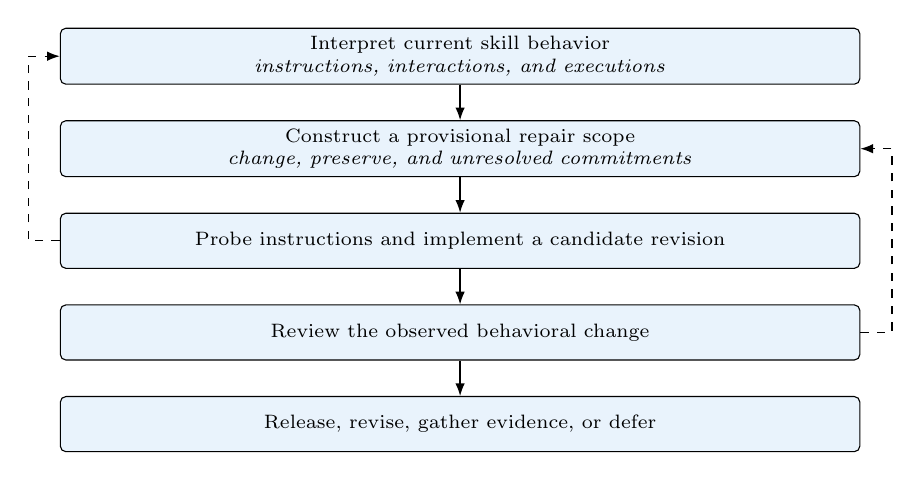
\begin{tikzpicture}[
        node distance=4.5mm,
        every node/.style={font=\scriptsize,align=center},
        box/.style={draw,rounded corners=2pt,fill=draftblue,
                   text width=0.82\columnwidth,minimum height=7mm,inner sep=3pt},
        arrow/.style={-{Latex[length=1.6mm]},line width=0.45pt}
    ]
        \node[box] (a) {Interpret current skill behavior\\
        \emph{instructions, interactions, and executions}};
        \node[box,below=of a] (b) {Construct a provisional repair scope\\
        \emph{change, preserve, and unresolved commitments}};
        \node[box,below=of b] (c) {Probe instructions and implement a candidate revision};
        \node[box,below=of c] (d) {Review the observed behavioral change};
        \node[box,below=of d] (e) {Release, revise, gather evidence, or defer};
        \draw[arrow] (a) -- (b);
        \draw[arrow] (b) -- (c);
        \draw[arrow] (c) -- (d);
        \draw[arrow] (d) -- (e);
        \draw[arrow,dashed] (d.east) -- ++(4mm,0) |- (b.east);
        \draw[arrow,dashed] (c.west) -- ++(-4mm,0) |- (a.west);
    \end{tikzpicture}
    \caption{Provisional process model to retain only if supported by the final
    analysis. Evidence can revise both the presumed instruction relationship and
    the intended scope of repair.}
    \Description{A vertical five-stage process: interpret current skill behavior, construct repair scope, probe instructions and implement a candidate, review behavioral change, and choose release, revision, more evidence, or deferral. Dashed arrows return from later stages to earlier interpretation and scoping.}
    \label{fig:repair-process}
\end{figure}

\subsection{Design Goals for Behavioral Patch Review}
\label{sec:formative-dgs}

We synthesized three design goals for supporting skill repair when runtime
behavior and the desired policy remain only partially understood.

\paragraph{DG1: Connect skill text to execution evidence.}
The interface should help users relate skill instructions and edits to behavior
across repeated executions. Task context and tool results provide controlled
inputs for these comparisons, and each summary should remain linked to its
executed intervention and raw runs [F1].

\paragraph{DG2: Make the repair scope explicit and revisable.}
The interface should help workflow owners articulate where a repair should
change behavior, preserve established behavior, or leave a policy unresolved.
These commitments should be grounded in concrete cases and remain editable as
new executions refine the owner's interpretation. The resulting scope serves
as both an evolving specification and the reference for reviewing a candidate
[F1, F2].

\paragraph{DG3: Support evidence-grounded review while preserving release authority.}
AI may generate cases, run probes, organize comparisons, and draft revisions.
Workflow owners should be able to see how their behavioral scope guides the
textual implementation and how the complete revision changes observable
decisions, tool actions, and outcomes. The workflow should culminate in a choice
to release, revise, gather more evidence, or defer [F2, F3].

Together, these goals motivate \emph{behavioral patch review}: a shared workflow
that connects user judgments, reusable skill instructions, execution evidence,
and enacted behavior. The next section describes how \systemname{}
operationalizes this process.

\section{\systemname: Behavioral Patch Review for Skills}
\label{sec:system}

\systemname{} supports skill repair as a review of three related changes. The
\emph{intended behavioral delta} describes what a workflow owner wants to
change, preserve, or leave unresolved. The \emph{artifact delta} is the
revision encoded in the skill. The \emph{enacted behavioral delta} is the
change observed when the original and revised skills are executed in
comparable situations. A repair becomes reviewable when these three deltas can
be examined together rather than inferred from a textual edit or a successful
rerun of the motivating incident alone.

Figure~\ref{fig:system-overview} summarizes the interaction. The owner first
constructs a behavioral scope from concrete cases. The system then organizes
evidence that relates this scope to the current skill and to a candidate
revision. Matched executions make the behavioral reach of the candidate
visible before the owner decides whether to release it. These activities are
iterative: evidence may prompt a revision to the intended scope, the skill, or
the cases considered relevant. The system therefore provides a shared review
record rather than treating repair as a one-shot generation task.

\begin{figure*}[t]
    \centering
    \small
    \setlength{\tabcolsep}{4pt}
    \begin{tabular}{@{}C{0.225\textwidth} C{0.225\textwidth} C{0.225\textwidth} C{0.225\textwidth}@{}}
        \fbox{\begin{minipage}[t][3.55cm][t]{0.205\textwidth}
            \textbf{1. Articulate intent}\\[3pt]
            Examine the failure and nearby cases\\
            Record behavior to change, preserve,\\
            or leave unresolved\\[4pt]
            Construct the intended behavioral delta.
        \end{minipage}}
        &
        \fbox{\begin{minipage}[t][3.55cm][t]{0.205\textwidth}
            \textbf{2. Assemble evidence}\\[3pt]
            Relate commitments to source regions\\
            Inspect relevant executions\\
            Review evidentiary limits\\[4pt]
            Connect intent to the current skill.
        \end{minipage}}
        &
        \fbox{\begin{minipage}[t][3.55cm][t]{0.205\textwidth}
            \textbf{3. Inspect the revision}\\[3pt]
            Generate, edit, or import a candidate\\
            Review the textual delta with links\\
            to intent and evidence\\[4pt]
            Make the artifact delta legible.
        \end{minipage}}
        &
        \fbox{\begin{minipage}[t][3.55cm][t]{0.205\textwidth}
            \textbf{4. Review enacted change}\\[3pt]
            Compare original and revised behavior\\
            Identify intended effects, regressions,\\
            and unresolved boundaries\\[4pt]
            Release, revise, investigate, or defer.
        \end{minipage}}
    \end{tabular}
    \caption{\systemname{} makes the intended, artifact, and enacted deltas
    jointly reviewable. Evidence connects the owner's behavioral scope to the
    current skill and candidate revision; matched executions support revision
    and release decisions.}
    \Description{Four panels show articulating intended behavior, assembling
    execution evidence, inspecting a skill revision, and reviewing enacted
    behavioral change before a release decision.}
    \label{fig:system-overview}
\end{figure*}

\subsection{Interaction Overview}
\label{sec:system-walkthrough}

We illustrate the workflow through Lin, the researcher introduced in
Section~\ref{sec:introduction}. Her travel-recovery skill selected an
inexpensive replacement flight that arrived after a fixed conference
presentation. The execution was plainly unacceptable, but it did not by
itself establish the policy that should govern future disruptions.

Lin begins by expressing the desired change in her own terms: fixed
commitments should take priority over price. \systemname{} places this incident
alongside neighboring cases that expose the reach of such a rule. Lin wants to
retain cost sensitivity for routine travel and confirmation before a
consequential purchase, while leaving an extreme fare trade-off unresolved.
Together, these judgments turn an objection to one outcome into a provisional
behavioral scope.

The system next brings together relevant parts of the current skill and
evidence from controlled executions. A targeted source intervention suggests
that an instruction treating calendar conflicts as a soft trade-off is
behaviorally relevant in the incident. The result is presented as bounded
evidence about sensitivity to a source region, not as proof of unique causal
responsibility or validation of a future revision. Lin can revise her scope if
this evidence changes her interpretation of the problem.

An AI service then drafts a candidate from the current skill, Lin's recorded
scope, and the reviewed evidence. \systemname{} presents the candidate as a
line-based diff. Annotations connect each changed block to the behavioral
commitment it is intended to address and to the evidence that informed the
revision. These links make the rationale and provenance of the artifact delta
inspectable without implying that a textual change has achieved its intended
effect.

Finally, \systemname{} executes the complete original and revised skills on
the reviewed cases under matched conditions. Lin can see whether the incident
is repaired, whether valued behaviors are preserved, and whether the revision
enters a boundary for which she has not yet defined a policy. She may revise
the skill or behavioral scope, request further evidence, defer the repair, or
release the reviewed version. The same scope therefore links her initial
intent to the textual revision, enacted outcomes, and final decision.

\subsection{Defining the Behavioral Scope of a Skill Repair}
\label{sec:behavioral-scope}

A review begins with an observable breakdown, the active skill, and the
available execution record. \systemname{} brings the task context, skill
instructions, tool activity, decisions, and outcome into a common view. This
reconstruction helps the owner distinguish what the skill said from what the
agent enacted and provides a stable point of comparison for later evidence.

The owner constructs a behavioral scope from the motivating incident,
accepted prior behavior, and contrastive cases. Each case $c$ combines a task
context, baseline evidence $B_0(c)$, and one of three normative dispositions:

\begin{itemize}[leftmargin=*]
    \item \textsc{Change}$(g_c)$ identifies behavior the revision should
    produce, such as selecting an itinerary that arrives before a fixed
    presentation.
    \item \textsc{Preserve}$(p_c)$ identifies a valued property that should
    remain stable, such as requesting confirmation before a consequential
    purchase.
    \item \textsc{Unresolved} marks a policy boundary for which the owner is
    not yet prepared to authorize a general rule, such as the acceptable fare
    premium for protecting a commitment.
\end{itemize}

Cases that are relevant to monitoring but outside the current repair can be
kept outside the candidate author's normative input. If a revision changes one
of these cases, the system returns it to the owner for judgment rather than
treating it as evidence of success or failure. This distinction separates
uncertainty about policy from evidence that an authorized commitment was met.

Commitments can concern decisions, tool calls, action ordering, confirmation
points, or outcomes. Each is paired with an observable criterion that the
owner can inspect. The system preserves successive versions of the scope so
that later evidence can be interpreted against the commitments that were in
place when a candidate was produced.

\paragraph{Scope anchors and contrastive cases.}
The motivating incident anchors the repair, but nearby cases clarify its
intended reach. These cases can come from prior executions, examples supplied
by the owner, or system-generated contrasts reviewed by the owner. Each
contrast makes explicit how it differs from an existing case and which policy
boundary it probes. This comparative representation allows a vague request
such as ``prioritize important events'' to become a set of concrete, revisable
commitments without requiring the owner to author a complete policy upfront.

\paragraph{Pre-reveal boundary commitments.}
Where possible, the owner records these commitments before seeing candidate
outcomes. This ordering preserves a prospective account of intended behavior
rather than allowing the observed candidate to redefine the repair
retrospectively. Selected cases may also remain outside an AI author's input,
allowing later executions to examine whether the revision extends beyond the
examples that directly informed it. These cases do not certify generalization;
they provide bounded evidence about the reach of the reviewed repair.

\subsection{Locating Source Instructions and Reviewing the Repair Preview}
\label{sec:instruction-effects}

To help the owner relate an observed breakdown to the skill, \systemname{}
supports targeted interventions on an isolated copy of the source artifact. A
model-assisted planner identifies an instruction and an already reconstructed
case that are relevant to the current scope; the execution service then
compares the original behavior with behavior under bounded variants of that
instruction. The reviewed skill itself is not changed during this process.

The resulting evidence answers a deliberately narrow question: under the
selected case and execution conditions, is observable behavior sensitive to
this source region? It does not establish unique causality, capture
interactions among all instructions, or validate text that has not yet been
executed. \systemname{} keeps this limitation visible and retains links to the
underlying artifact versions, cases, executions, and observable differences.

The repair preview places this source-location evidence alongside the owner's
behavioral scope. Its purpose is to let the owner review the evidence and
commitments that will inform implementation, not to ask them to approve a
system-generated policy. The owner can return to the scope whenever the
evidence reveals that the intended repair was underspecified. Exact
interventions and execution budgets for the study instantiation are reported
in Appendix~\ref{app:probe-protocol}.

\subsection{Reviewing the Skill Diff and Its Behavioral Consequences}
\label{sec:candidate-review}

The workflow owner may write the candidate skill or delegate its
implementation to an AI service or collaborator. Regardless of authorship,
\systemname{} records the candidate as a revision of the current skill and
associates it with the behavioral scope and evidence available at the time.
This provenance preserves the distinction between deciding what behavior is
acceptable and choosing text intended to produce it.

The primary artifact view uses a familiar line-based review layout. Added and
removed skill text is accompanied by compact annotations that distinguish four
kinds of information:

\begin{itemize}[leftmargin=*]
    \item \textbf{Scope commitment} identifies the intended behavior that a
    changed block is meant to address.
    \item \textbf{Implementation rationale} records why the candidate author
    associated that text with the commitment.
    \item \textbf{Source evidence} shows execution evidence that made the
    corresponding region of the original skill relevant to the repair.
    \item \textbf{Candidate evidence}, when available, reports bounded
    evidence about the behavioral sensitivity of the revised block.
\end{itemize}

The annotations support navigation between the behavioral and textual objects
of review; they do not attribute a whole-candidate outcome to a single edited
block. Evidence about the source skill, an optional intervention on candidate
text, and execution of the complete candidate therefore remain visibly
distinct.

After a candidate is committed, \systemname{} executes the complete original
and revised skills on the reviewed cases. For case $c$, it estimates candidate
behavior $B_p(c)$ under conditions matched to the baseline $B_0(c)$, including
task context, tool state, model configuration, and side-effect policy. The
comparison evaluates the candidate as a whole and organizes the result into
four review states:

\begin{table}[t]
    \caption{Primary review states and their meanings.}
    \label{tab:review-states}
    \small
    \begin{tabularx}{\columnwidth}{@{}p{0.25\columnwidth}Y@{}}
        \toprule
        \textbf{State} & \textbf{Meaning} \\
        \midrule
        Aligned & Available evidence is consistent with a recorded Change or Preserve commitment. \\
        Mismatch & A desired change remains unmet or a valued behavior regresses. \\
        Needs judgment & The candidate changes behavior in a region for which the owner has not authorized a target. \\
        Insufficient evidence & The available executions do not support a stable comparison. \\
        \bottomrule
    \end{tabularx}
\end{table}

The workspace gives priority to mismatches, unresolved changes, and
insufficient evidence while keeping commitments separate. Repairing the
motivating incident therefore cannot conceal a regression in a behavior the
owner intended to preserve. Cross-highlighting connects a selected case to its
commitment, whole-candidate outcome, and related skill blocks, helping the
owner move between intended, artifact, and enacted deltas.

When a result remains difficult to interpret, the owner can inspect individual
executions, gather additional evidence, or request a bounded intervention on a
candidate block. These actions provide further evidence without converting an
unresolved policy question into an automated judgment. The owner can then edit
the candidate, revise the scope, defer the repair, or release the reviewed
version. Cases and criteria accepted during review can inform future
regression checks.

\paragraph{Behavior evaluation.}
The evaluated prototype represents behavior through observable tool traces and
environment outcomes. Fact criteria capture properties such as arrival time or
ledger creation; trace criteria capture events and ordering, such as
confirmation preceding booking. In the controlled study, confirmatory outcomes
use deterministic rules over these reconstructable records rather than an LLM
semantic judge. Cases without an authorized target are evaluated only for
material behavioral change and returned to the owner for judgment. The system
stores observable traces and outcomes, not hidden chain-of-thought.

\subsection{System Architecture, Implementation, and Scope}
\label{sec:system-implementation}

\systemname{} is implemented as a web-based review workspace backed by an
orchestration service. A skill comprises natural-language instructions, a
typed tool interface, and an execution configuration. Each execution receives
an isolated copy of a stateful tool environment, allowing the system to expose
realistic decisions, tool results, and side effects without reaching a
production account. Original, intervened, and candidate skills are retained as
separate versions so that evidence can be traced to the artifact and context
that produced it.

LLM services perform bounded interpretive and generative work: they help
retrieve relevant cases, propose source regions for inspection, draft
candidate revisions, and explain computed comparisons. They do not fabricate
tool results, modify recorded owner commitments, determine confirmatory
outcomes, or authorize release. Execution and evaluation services maintain
these boundaries by validating tool calls against the scenario environment and
computing study outcomes from observable traces and end states.

The study instantiation freezes model configurations, scenario worlds,
candidate-generation inputs, and execution budgets within each condition.
It also records the provenance of scope revisions, candidate versions,
executions, and release decisions. These controls support matched comparisons
and reconstruction of a review without turning the product interaction into an
experiment-specific sequence. Appendix~\ref{app:system-details} reports the
data model, intervention protocol, execution configuration, and prompt
contracts used in the evaluated prototype.

\systemname{} provides bounded evidence about a revision rather than a
guarantee of behavior outside the reviewed cases and execution conditions.
Targeted interventions indicate sensitivity, not unique causal responsibility;
matched executions characterize the complete candidate only within the
observed contexts. The workflow therefore retains explicit states for
unresolved policy and insufficient evidence, and allows the owner to keep the
current skill whenever a revision is not yet justified.

\section{Technical Evaluation}
\label{sec:technical-evaluation}

Behavioral patch review depends on execution evidence that is sufficiently
faithful and stable for a workflow owner to interpret. We therefore evaluated
the evidence pipeline separately from the user study. The evaluation asks
whether the prototype reconstructs observable behavior correctly, whether its
matched comparisons remain stable under the frozen study configuration, and
whether targeted source interventions provide useful discrimination without
being mistaken for proof of causality.

\subsection{Evaluation Questions and Corpus}

We organized the evaluation around three technical questions:

\begin{description}[leftmargin=0pt,labelindent=0pt,style=nextline]
    \item[\textbf{TQ1: Evidence fidelity.}] Do the trace and fact evaluators
    accurately reconstruct the decisions, tool actions, and outcomes relevant
    to each behavioral commitment?
    \item[\textbf{TQ2: Execution stability.}] Do repeated executions of the
    same skill and case support a stable matched comparison under the study
    configuration?
    \item[\textbf{TQ3: Intervention discriminability.}] Do bounded
    interventions expose sensitivity to repair-relevant source regions while
    preserving a visible distinction between source-location evidence and
    whole-candidate validation?
\end{description}

The evaluation corpus contains the complete travel-recovery and
expense-review scenario packs used in the controlled study. Each pack includes
the faulty source skill, an independently authored reference repair, the
product-facing cases, post-decision cases, typed tool schemas, and frozen world
states. Reference behaviors and case-level criteria were specified before the
candidate-generation path was sampled. We exercised the faulty skill,
reference repair, source interventions, and end-to-end candidate path across
all cases using the same model and execution service later used in the study.
Appendix~\ref{app:system-details} reports the exact artifacts, budgets, and
configuration.

\subsection{Measures and Analysis}

For evidence fidelity, two researchers independently inspected a stratified
sample of raw tool traces and terminal world states and annotated the
commitment-relevant facts and event ordering. We compared these annotations
with the system's deterministic evaluator outputs, resolving disagreements
without access to condition labels or candidate provenance. We report exact
agreement, class-specific errors, and inter-rater agreement before resolution.

For execution stability, we measured valid-run rate, modal behavior share, and
agreement of commitment-relevant facts across repetitions of each
skill--case pair. We examined the faulty and reference artifacts separately so
that a stable evaluator could not conceal unstable agent behavior. For matched
comparisons, we additionally verified that original and candidate executions
shared the same task context, tool snapshot, configuration, and side-effect
policy.

For intervention discriminability, we compared the selected source
interventions with interventions on instructions not expected to govern the
target behavior. We measured whether each intervention changed the incident's
commitment-relevant facts, whether it also altered preservation cases, and how
often the selected source region ranked above non-target regions by behavioral
sensitivity. This analysis evaluates the usefulness of the cue under the
scenario corpus; it does not estimate unique causal responsibility among
interacting natural-language instructions.

Finally, we sampled the complete candidate-generation and execution path to
test whether the evidence shown during a realistic repair remained
reconstructable end to end. We report incident success, preservation and
holdout behavior, execution failures, and operational latency. These candidate
samples assess the readiness of the study apparatus rather than the human
benefit of the workspace.

\subsection{Results}

\paragraph{TQ1: Evaluators faithfully reconstructed observable behavior.}
Across \DataNeeded{NUMBER OF MANUALLY AUDITED EXECUTIONS} audited executions,
the deterministic evaluators agreed with the resolved human annotations on
\DataNeeded{OVERALL EXACT AGREEMENT, WITH CONFIDENCE INTERVAL}. Agreement was
\DataNeeded{FACT-CRITERION AGREEMENT} for fact criteria and
\DataNeeded{TRACE-ORDER AGREEMENT} for trace-order criteria. Independent
annotators achieved \DataNeeded{INTERRATER AGREEMENT AND MEASURE} before
resolution. The remaining \DataNeeded{NUMBER} discrepancies involved
\DataNeeded{CHARACTERIZE EXTRACTION OR TRACE-ORDER EDGE CASES}; none
\DataNeeded{CONFIRM WHETHER ANY DISCREPANCY CHANGED A CASE-LEVEL REVIEW STATE}.
We corrected \DataNeeded{REPORT ANY EVALUATOR OR FIXTURE CORRECTIONS MADE
BEFORE FREEZING THE STUDY BUILD} and repeated the affected calibration before
participant data collection.

\paragraph{TQ2: Matched executions were stable enough to expose genuine
uncertainty.}
The frozen corpus produced valid executions in
\DataNeeded{VALID-RUN RATE AND NUMERATOR/DENOMINATOR}. Commitment-relevant
behavior was stable in \DataNeeded{NUMBER OR PROPORTION OF SKILL--CASE PAIRS
MEETING THE PREREGISTERED STABILITY THRESHOLD}, with a median modal share of
\DataNeeded{MEDIAN AND INTERQUARTILE RANGE}. The faulty skills reliably
reproduced the motivating breakdowns, while the reference repairs achieved
their incident targets and preservation criteria in
\DataNeeded{REFERENCE SUCCESS RATES}. The remaining unstable pairs concerned
\DataNeeded{CHARACTERIZE UNSTABLE CASES}; the interface surfaced these as
insufficient evidence rather than collapsing them into a deterministic
outcome. Configuration audits found \DataNeeded{NUMBER} unmatched original--
candidate comparisons after freezing \DataNeeded{EXPECTED TO BE ZERO; REPORT
ANY EXCEPTIONS AND THEIR HANDLING}.

\paragraph{TQ3: Source interventions provided discriminating but bounded
location cues.}
The source regions selected for the two scenario packs changed the
incident-relevant behavior in \DataNeeded{SELECTED-INTERVENTION HIT RATE},
compared with \DataNeeded{NON-TARGET INTERVENTION RATE} for non-target source
regions. They ranked within the top \DataNeeded{RANK OR PERCENTILE} regions by
behavioral sensitivity in \DataNeeded{PROPORTION OF CALIBRATION SAMPLES}.
Their effects were not perfectly local: \DataNeeded{NUMBER OR PROPORTION} also
changed at least one neighboring case, illustrating why the system treats the
intervention as a source-location cue and subsequently executes the complete
candidate across the behavioral scope. No source intervention result was used
as confirmatory evidence for newly generated text.

\paragraph{The complete candidate path supported the planned study tasks.}
Across \DataNeeded{NUMBER OF END-TO-END CANDIDATE SAMPLES}, generated
candidates repaired the motivating incident in
\DataNeeded{INCIDENT SUCCESS RATE}, preserved visible commitments in
\DataNeeded{VISIBLE PRESERVATION RATE}, and preserved generator-withheld
behavior in \DataNeeded{WITHHELD PRESERVATION RATE}. The candidate path also
produced \DataNeeded{NUMBER AND TYPES OF DELIBERATE OR NATURALLY OCCURRING
MISMATCHES} cases in which review should lead to revision, further evidence, or
deferral rather than release. Median end-to-end latency was
\DataNeeded{LATENCY WITH DISTRIBUTION}, and execution or service failures
occurred in \DataNeeded{FAILURE RATE}. These results established that both
study conditions could expose the same substantive repair evidence within the
planned task duration.

\subsection{Summary and Evidentiary Boundaries}

The technical evaluation supports the use of deterministic trace and fact
evidence for the two controlled domains and shows that the prototype can
distinguish stable behavior from insufficient evidence. It also supports the
narrower role assigned to source interventions: they can direct attention to
behaviorally relevant text, but their effects may extend across cases and do
not identify a unique causal instruction. The evaluation does not establish
reliability for arbitrary skills, tools, models, or deployment environments.
The controlled user study therefore tests whether people benefit from this
evidence within the evaluated scope, not whether \systemname{} certifies a
revision for unrestricted use.

\section{Controlled User Study}
\label{sec:user-study}

We conducted a controlled study to examine whether behavioral patch review
helps workflow owners understand and govern a skill repair relative to a
capability-matched conversational interface. The comparison concerns how
repair work is represented and reviewed, rather than the presence of any
single interface control. We evaluated the complete interaction model because
its contribution lies in connecting intent, artifact revision, and enacted
behavior; the study does not estimate the isolated effect of each workspace
component.

\subsection{Research Questions and Conditions}

The study addressed three research questions:

\begin{description}[leftmargin=0pt,labelindent=0pt,style=nextline]
    \item[\textbf{RQ1: Behavioral understanding.}] Does the structured
    workspace help owners understand the enacted behavioral change produced by
    a candidate revision?
    \item[\textbf{RQ2: Repair scope.}] Does it help owners construct and
    maintain a repair scope across intended changes, valued behavior, and
    unresolved boundaries?
    \item[\textbf{RQ3: Release judgment.}] Does it support decisions that are
    better calibrated to the available evidence while preserving the owner's
    authority over release?
\end{description}

In the \emph{workspace} condition, behavioral commitments, the skill
revision, and matched execution evidence remain persistently visible and
cross-linked. In the \emph{chat} condition, participants can access the same
skill, cases, evidence-generating operations, and revision capabilities
through conversation, but these objects are presented sequentially rather
than integrated into a persistent review representation. Both conditions ask
participants to make the same substantive judgments about the motivating
incident, neighboring cases, candidate revision, and final disposition.

The two conditions use the same underlying model, candidate-generation
process, typed tool runtime, scenario worlds, case exposure, outcome criteria,
and execution budgets. Interface organization is therefore the primary
manipulation: the workspace externalizes relationships among intent, artifact,
and enacted behavior, whereas the chat condition requires participants to
maintain and reconcile those relationships through the conversation. Exact
configurations and execution protocols are reported in
Appendix~\ref{app:system-details}.

\subsection{Design, Tasks, and Assignment}

We used a counterbalanced within-participant design with two domains:
travel-disruption rebooking and expense-receipt review. Each participant
completed one task in each condition and encountered each domain only once,
avoiding direct repetition of the same repair problem. Four assignment
sequences balanced condition order, domain order, and condition--domain
mapping. We determined the final sample size through
\DataNeeded{DESCRIBE THE A PRIORI POWER ANALYSIS, TARGET EFFECT, POWER, AND
ALLOWANCE FOR EXCLUSIONS} after a usability pilot whose participants did not
enter confirmatory analyses.

Each task placed the participant in the role of a workflow owner responsible
for reviewing a problematic execution and deciding whether a revised skill is
ready for reuse. The scenario includes the motivating incident, visible
contrastive cases that probe desired changes and preservation constraints, a
policy boundary, and cases reserved for post-decision assessment. Selected
cases were withheld from candidate generation to distinguish direct repair of
visible examples from transfer to behavior that did not guide the revision.
Both conditions disclosed that all actions occurred in an isolated
environment, but neither revealed the injected fault, a reference repair, or
the hidden assessment criteria.

\subsection{Participants}

We recruited \StudyN{} adults who
\DataNeeded{REPORT ELIGIBILITY CRITERIA, INCLUDING EXPERIENCE WITH LLM TOOLS,
RECURRING WORKFLOWS, OR REVIEW OF AUTOMATED OUTPUTS}. We did not require
participants to program or directly author an agent skill because the target
role was the person responsible for acceptable behavior and release. The
sample included \DataNeeded{REPORT AGE SUMMARY, GENDER ONLY AS COLLECTED,
EDUCATION OR OCCUPATIONAL BACKGROUND, LLM EXPERIENCE, AND RELEVANT DOMAIN
EXPERIENCE}. \DataNeeded{REPORT WHETHER AND HOW MANY PARTICIPANTS HAD PRIOR
EXPERIENCE EDITING PROMPTS, SKILLS, OR AUTOMATIONS}.

Participants received \StudyCompensation{} for a session lasting
\DataNeeded{PLANNED AND OBSERVED SESSION DURATION}. The study was reviewed
under \StudyEthics{}. We excluded \DataNeeded{NUMBER} participants according
to the preregistered criteria because \DataNeeded{REPORT EXCLUSION REASONS};
\DataNeeded{NUMBER} completed participant records entered the confirmatory
analysis. A separate \DataNeeded{PILOT N} participants completed the usability
pilot and were not included in the reported results.

\subsection{Procedure}

Each task followed four phases shared across conditions. First, participants
inspected the skill and a recurring execution failure, then described what
should have happened. Second, they examined contrastive cases and recorded
whether the revision should change the observed behavior, preserve it, or
leave the policy boundary unresolved. These judgments established a
prospective repair scope before candidate outcomes were available.

Third, participants reviewed bounded evidence connecting the current behavior to
the source skill and inspected a candidate revision produced from the same
information in both conditions. They then compared the complete original and
revised skills across the reviewed cases. Participants could inspect
underlying executions, edit or regenerate the candidate, request further
evidence, revise their scope, defer the repair, or release the candidate. The
interface recorded scope changes made after outcomes became visible so that
they could be distinguished from pre-reveal commitments.

Finally, before a previously unseen case was executed, participants predicted
observable aspects of the candidate's behavior and reported their confidence.
They then completed experience and workload measures. The final artifact was
evaluated on the prediction case and on a research holdout that was unavailable
during the task. These post-decision cases assessed behavioral understanding
and transfer without changing the participant's completed release decision.

\subsection{Measures}

We preregistered three co-primary outcomes aligned with the research questions
\DataNeeded{PROVIDE PREREGISTRATION REFERENCE AND STATE ANY DEVIATIONS}.
\emph{Held-out behavioral understanding} combines accuracy on observable
predictions about a previously unseen case with calibration derived from
participants' confidence. \emph{Behavioral-scope adherence} measures the
proportion of pre-reveal Change and Preserve commitments satisfied by the final
candidate; cases intentionally left unresolved do not enter this denominator.
\emph{Evidence-calibrated decision quality} assesses whether the terminal
action and its rationale are supported by the evidence available at the time.
A release is unsupported when an unmet change target, preservation regression,
execution failure, or material evidence gap remains; a decision not to release
is evidence-grounded when it identifies a remaining mismatch, unresolved
consequence, or evidentiary limitation. A change within an unresolved boundary
requires acknowledgement but is not treated as an error by default.

Secondary outcomes characterized both repair quality and interaction process.
They included incident resolution, preservation of visible and generator-
withheld behavior, performance on the blind holdout, identification of case
roles, regression detection, task time, evidence requests, candidate and scope
revisions, release path, and consequential failures. Post-task items measure
participants' understanding of the original and revised skills, ability to
anticipate behavior, awareness of repair boundaries, perceived sufficiency of
evidence, explainability of the final decision, and perceived control. We also
collected the six Raw TLX dimensions and report them separately.

\subsection{Analysis and Data Integrity}

Confirmatory models included condition, domain, period, and order as fixed
effects and participant as a random intercept. We used mixed-effects models
appropriate to binary, continuous, and count outcomes, applied the
preregistered multiplicity procedure to the three co-primary outcomes, and we
report effect sizes with confidence intervals. The two domains were treated as
fixed task contexts, not as a random sample of all possible agent workflows.

The system recorded the skill and scope versions, timing of outcome reveals,
candidate provenance, execution traces, evidence requests, and terminal
decision for each task. This record supports reconstruction of the evidence
available to a participant without exposing reference repairs or hidden
holdouts during the interaction. Questionnaire responses were joined to this
record only after the task was complete.

Before confirmatory data collection, we completed technical acceptance,
calibrated the faulty and reference behaviors across all study cases, tested
the end-to-end candidate path, audited both conditions for information
leakage, and conducted a separate usability pilot. We then froze the study
build; \DataNeeded{REPORT ANY POST-FREEZE DEVIATIONS OR STATE THAT NONE
OCCURRED}. Appendix~\ref{app:system-details} documents the exact configuration
and reconstruction protocol.

\subsection{Results}

\begin{table*}[t]
    \caption{Co-primary outcomes by condition. Values and model estimates are
    placeholders pending the confirmatory analysis. Higher values indicate
    better performance for prediction accuracy and scope adherence; lower
    Brier scores indicate better calibrated predictions.}
    \label{tab:user-study-primary}
    \small
    \begin{tabularx}{\textwidth}{@{}p{0.25\textwidth}Y Y Y@{}}
        \toprule
        \textbf{Outcome} & \textbf{Workspace} & \textbf{Chat} &
        \textbf{Condition effect} \\
        \midrule
        Held-out prediction accuracy &
        \DataNeeded{ESTIMATE AND CI} &
        \DataNeeded{ESTIMATE AND CI} &
        \DataNeeded{MODEL EFFECT, CI, ADJUSTED P} \\
        Prediction calibration (Brier) &
        \DataNeeded{ESTIMATE AND CI} &
        \DataNeeded{ESTIMATE AND CI} &
        \DataNeeded{MODEL EFFECT, CI, ADJUSTED P} \\
        Behavioral-scope adherence &
        \DataNeeded{ESTIMATE AND CI} &
        \DataNeeded{ESTIMATE AND CI} &
        \DataNeeded{MODEL EFFECT, CI, ADJUSTED P} \\
        Evidence-calibrated decision quality &
        \DataNeeded{ESTIMATE AND CI} &
        \DataNeeded{ESTIMATE AND CI} &
        \DataNeeded{MODEL EFFECT, CI, ADJUSTED P} \\
        \bottomrule
    \end{tabularx}
\end{table*}

\paragraph{Task completion and condition integrity.}
Participants completed \DataNeeded{NUMBER OF ANALYZED TASKS} analyzed tasks.
\DataNeeded{REPORT INTERRUPTIONS, RESUMED TASKS, EXECUTION FAILURES, AND ANY
MISSING QUESTIONNAIRES}. Audit records confirmed that the two conditions used
the same scenario artifacts, candidate-generation inputs, execution evidence,
and outcome criteria in \DataNeeded{PROPORTION OF TASKS; EXPLAIN ANY
DEVIATIONS}. The manipulation check showed that participants experienced the
workspace as a more persistent and connected representation of the repair
\DataNeeded{REPORT ITEM OR CHECK, EFFECT, CI, AND P}, while access to the skill,
cases, and repair operations did not differ substantively
\DataNeeded{REPORT CAPABILITY-PARITY CHECK}. We found
\DataNeeded{REPORT PERIOD, ORDER, AND DOMAIN EFFECTS, INCLUDING ANY
CONDITION--DOMAIN INTERACTION}.

\paragraph{RQ1: The workspace improved understanding of enacted behavioral
change.}
Participants predicted behavior on the previously unseen case more accurately
in the workspace condition than in chat (Table~\ref{tab:user-study-primary}).
The estimated difference was \DataNeeded{PREDICTION-ACCURACY EFFECT, CI,
ADJUSTED P, AND EFFECT SIZE}. Their confidence was also better calibrated:
selected-answer Brier scores were lower by \DataNeeded{BRIER EFFECT, CI,
ADJUSTED P}. \DataNeeded{REPORT WHETHER THE BENEFIT CAME FROM CORRECTLY
ANTICIPATING DECISIONS, TOOL ACTIONS, CONFIRMATION ORDER, OUTCOMES, OR A
COMBINATION}.

The behavioral prediction result was consistent with participants' experience
ratings. They reported greater understanding of the candidate
\DataNeeded{ITEM ESTIMATE, EFFECT, CI, P} and greater ability to anticipate its
behavior \DataNeeded{ITEM ESTIMATE, EFFECT, CI, P}. Interaction records suggest
that workspace participants used the cross-links among cases, commitments, and
the skill diff to reconstruct why behavior changed
\DataNeeded{REPORT RELEVANT NAVIGATION OR EVIDENCE-VIEWING PATTERN}. In chat,
participants more often requested or produced repeated summaries of earlier
cases \DataNeeded{COUNT OR PROPORTION AND COMPARISON}, indicating that the same
evidence was harder to maintain as a single review object. A participant
described the contrast as \emph{``\DataNeeded{VERIFIED POST-TASK QUOTE ABOUT
CONNECTING THE REVISION TO BEHAVIOR ACROSS CASES}.''}

\paragraph{RQ2: The workspace produced repairs that better respected their
prospective scope.}
Final candidates in the workspace condition satisfied a greater proportion of
the participants' pre-reveal Change and Preserve commitments
\DataNeeded{SCOPE-ADHERENCE EFFECT, CI, ADJUSTED P, AND EFFECT SIZE}. Incident
success was \DataNeeded{WORKSPACE AND CHAT RATES}, while preservation of
visible behavior was \DataNeeded{WORKSPACE AND CHAT RATES}. The difference was
especially apparent on the generator-withheld Preserve case
\DataNeeded{TRANSFER EFFECT, CI, P}, which did not directly inform candidate
generation. Blind-holdout performance showed \DataNeeded{REPORT DIRECTION,
MAGNITUDE, CI, AND WHETHER THE RESULT WAS CONFIRMATORY OR EXPLORATORY}.

Participants using the workspace identified more preservation regressions
before their terminal decision \DataNeeded{EFFECT, CI, P} and were more likely
to acknowledge a material change in an Unresolved case
\DataNeeded{EFFECT, CI, P}. They made \DataNeeded{WORKSPACE VERSUS CHAT SCOPE
REVISIONS} scope revisions after seeing candidate behavior. Inspection of
these revisions showed that \DataNeeded{REPORT HOW OFTEN THEY CLARIFIED A
GENUINE POLICY BOUNDARY VERSUS RETROFITTED INTENT TO THE CANDIDATE}. This
distinction is important: behavioral patch review supported revising an
underspecified scope, but did not treat post-reveal agreement as evidence that
the original repair had been well scoped.

\paragraph{RQ3: Release decisions were better calibrated to available
evidence.}
Workspace participants reached an evidence-supported terminal decision in
\DataNeeded{WORKSPACE RATE} of tasks, compared with \DataNeeded{CHAT RATE} in
chat \DataNeeded{MODEL EFFECT, CI, ADJUSTED P}. They released a candidate while
a recorded Change or Preserve mismatch remained in \DataNeeded{WORKSPACE RATE}
versus \DataNeeded{CHAT RATE} of eligible tasks, and they explicitly cited an
unresolved consequence or evidence limitation when declining release in
\DataNeeded{WORKSPACE RATE} versus \DataNeeded{CHAT RATE}. The result was not
simply greater reluctance to act: when the candidate satisfied the visible
scope and evidence was stable, workspace participants released it in
\DataNeeded{RATE}, compared with \DataNeeded{RATE} in chat.

Decision rationales in the workspace condition more often referred to both a
desired change and a preservation or boundary consideration
\DataNeeded{CODING PROCEDURE, AGREEMENT, RATES, EFFECT, AND P}. Participants
also reported greater evidence sufficiency \DataNeeded{EFFECT, CI, P},
decision explainability \DataNeeded{EFFECT, CI, P}, and perceived control
\DataNeeded{EFFECT, CI, P}. One participant summarized the division of labor:
\emph{``\DataNeeded{VERIFIED QUOTE ABOUT THE SYSTEM DOING EVIDENCE OR
IMPLEMENTATION WORK WHILE THE PARTICIPANT RETAINED THE RELEASE DECISION}.''}

\paragraph{Workload and interaction cost.}
The improvement in the co-primary outcomes did not require reliably longer
tasks: completion time differed by \DataNeeded{TIME EFFECT, CI, P}, with median
times of \DataNeeded{WORKSPACE MEDIAN} and \DataNeeded{CHAT MEDIAN}. Workspace
participants inspected \DataNeeded{MORE, FEWER, OR SIMILAR} distinct evidence
items and requested \DataNeeded{MODEL OR EXECUTION CALL COMPARISON}. Raw TLX
mental demand was \DataNeeded{DIRECTION, EFFECT, CI, P}; the remaining Raw TLX
dimensions showed \DataNeeded{REPORT PATTERN WITHOUT COLLAPSING DIMENSIONS INTO
AN UNJUSTIFIED COMPOSITE}. We observed \DataNeeded{NUMBER AND DESCRIPTION} tasks
in which the workspace's additional structure slowed an otherwise simple
repair, providing a boundary on when the interaction is beneficial.

\subsection{Study Summary}

Across two task domains, the results were consistent across the three
levels of behavioral patch review. The structured workspace improved
participants' ability to anticipate the enacted delta, helped their final
revision adhere to a prospectively recorded behavioral scope, and supported
terminal decisions that better reflected the available evidence. Process and
experience measures suggest that the benefit came from keeping cases,
commitments, skill changes, and executions available as one reviewable object,
rather than from providing additional agent capabilities. The study evaluates
the integrated interaction model and does not identify which individual visual
representation is necessary or sufficient for the observed effects.

\section{Discussion}
\label{sec:discussion}

The formative and evaluation results together reposition skill repair from
editing a natural-language artifact to governing a change in recurring agent
behavior. Participants could often recognize an unacceptable outcome before
they could state the reusable policy that should replace it. The system study
suggests that resolving this articulation gap requires more than an improved
text editor or a larger set of automatically generated tests. Workflow owners
benefited from keeping their intended behavioral delta, the candidate's
artifact delta, and its enacted behavioral delta available as related but
non-equivalent objects of review.

\subsection{The Unit of Review Is a Behavioral Change, Not a Textual Patch}

Code review works partly because the reviewed artifact has a comparatively
direct relationship to later execution. Natural-language skills weaken that
relationship: a small edit may interact with the task context, other
instructions, tool results, and model variation, while a substantial textual
change may leave observable behavior untouched. Existing prompt and agent
evaluation systems make important parts of this uncertainty testable
\cite{arawjo2024chainforge,kim2024evallm,sharma2025promptpex}, but their
comparison becomes most decisive once the desired behavior is sufficiently
specified.

Behavioral patch review instead treats the textual diff as one representation
within a larger review. The scope states the change the owner is prepared to
authorize; the artifact diff shows how that change was encoded; and matched
execution provides bounded evidence about what the candidate actually does.
The improvement in held-out prediction suggests that this organization helped
participants form a more operational understanding of the revision than the
same capabilities presented through chat. This is not evidence that textual
diffs are unhelpful. Rather, familiar artifact review becomes more useful when
it remains connected to the cases and executions that give the edited text
behavioral meaning.

This framing also changes what counts as a successful repair. Reproducing the
desired outcome in the incident is necessary but insufficient. A candidate is
reviewable only relative to behavior the owner intended to change, behavior
they intended to preserve, and boundaries for which no rule has yet been
authorized. The relevant unit is therefore a \emph{relative behavioral
change}, not an isolated outcome or a globally optimal skill.

\subsection{Repair Scope Is a Provisional Behavioral Specification}

The formative study showed that repair intent was constructed comparatively:
additional cases did not merely test a pre-existing policy, but exposed
preservation commitments and trade-offs that participants had not articulated
from the incident alone. The controlled study extends this observation. The
workspace produced stronger scope adherence and regression detection even
though both conditions had access to the same cases and agent operations. The
result suggests that cases can function as an interactive specification when
their relationships and normative status remain visible across revision and
execution.

This specification is deliberately provisional. \textsc{Change} and
\textsc{Preserve} express commitments that can be evaluated against observable
behavior, while \textsc{Unresolved} records the absence of an authorized rule.
Treating unresolved behavior as a first-class state avoids two common
collapses: allowing the candidate generator to silently settle a domain
trade-off, or forcing the owner to invent a complete policy before any
evidence is available. New executions may legitimately alter the scope, but
preserving pre-reveal judgments distinguishes learning from retrofitting the
specification to a candidate that has already been observed.

This account complements policy-authoring and test-generation systems
\cite{lam2025policymaps,lee2026dataprompt,koh2026contrastive}. A living test set
can evaluate a stable contract, whereas a behavioral scope also records how
the contract is still being negotiated. For reusable agents, future authoring
tools should therefore preserve the history and provenance of case-level
commitments, not only accumulate examples labeled successful or unsuccessful.

\subsection{Evidence Can Support Authority Without Replacing It}

Participants in the formative study distinguished work they were willing to
delegate from decisions they wanted to retain. They generally accepted AI
support for retrieving cases, running comparisons, and drafting skill text,
while treating acceptable policy and release as owner decisions. The user
study's decision results suggest that a structured evidence record can make
this division of labor operational: participants made decisions that more
closely reflected mismatches and evidence gaps without losing perceived
control.

The distinction is important because additional evidence is not equivalent to
additional authority. A source intervention may reveal sensitivity to one
instruction but cannot determine whether the resulting policy is acceptable.
Matched executions may show that a candidate crossed an unresolved boundary
but cannot resolve the underlying trade-off. Even a candidate that satisfies
every reviewed case may behave differently outside that scope. \systemname{}
therefore automates evidence and implementation work while preserving explicit
moments at which the owner must interpret, revise, or decline the proposed
change.

This design differs from both full automation and manual oversight of every
agent step. Full automation risks turning incomplete evidence into an implicit
policy, while continuous manual supervision undermines the value of reusable
agents. Behavioral patch review concentrates owner attention at consequential
boundaries: defining the intended change, inspecting conflicts between intent
and execution, and authorizing persistent reuse. In this sense, the system
supports governance through selective, evidence-grounded intervention rather
than permanent human involvement in each workflow.

\subsection{Implications for Reusable Agent Maintenance}

Our findings suggest four implications for systems that maintain reusable
agent artifacts. First, repair interfaces should preserve intent separately
from implementation. A candidate author can explain how text is meant to
address a commitment, but that rationale should not overwrite the owner's
wording or count as behavioral evidence. Second, systems should compare the
complete revised artifact under matched conditions. Local source or block
interventions can guide attention, but interactions among instructions make
whole-candidate execution the relevant basis for release review.

Third, evidence should retain its scope and provenance. Cases, artifact
versions, model and tool configurations, and exposure to candidate authors all
shape what a comparison can support. A compact interface may hide these fields
by default, but it should not detach summaries from reconstructable records.
Finally, release should create reusable review material rather than end the
process. Accepted Change and Preserve commitments can become regression cases,
while Unresolved cases remain visible boundaries for later evidence and policy
work.

Although we instantiate these implications through agent skills, the model may
apply to other natural-language artifacts that govern recurring behavior,
including system prompts, organizational policies, automation routines, and
agent templates. The key requirement is not a particular file format, but a
versionable control artifact whose effects can be observed across multiple
executions and judged by a person with authority over reuse. Determining how
behavioral patch review changes when authority is distributed across teams or
institutions remains an important direction for future work.

\section{Limitations and Future Work}
\label{sec:limitations}

Our results should be interpreted within the bounded settings in which the
system and studies were evaluated. The formative study examined
\DataNeeded{CHARACTERIZE THE PARTICIPANT POPULATION AND RANGE OF REPAIR
EPISODES}, and the controlled study placed participants in the role of a
workflow owner during two short, consequential but simulated tasks. This
design allowed us to compare conditions under matched evidence, but it does
not reproduce the accumulated context, organizational pressure, or delayed
consequences of maintaining an agent over weeks or months. Participants'
authority in the study was assigned by the task; in practice, the person
editing or approving a skill may not be the person most affected by its
behavior. Longitudinal deployments should examine how behavioral scopes and
release records evolve through repeated breakdowns and handoffs among owners,
maintainers, and affected stakeholders.

The controlled study used two fixed domains, one model configuration, typed
tool interfaces, and sandboxed world states. These choices provided
reconstructable outcomes and prevented study actions from affecting real
accounts. They also limit ecological and domain generality. Travel recovery
and expense review contain explicit decisions, constraints, and side effects;
skills for creative, interpersonal, or open-ended analytical work may not
admit equally clear fact or trace criteria. Future work should study domains in
which behavior must be reviewed through human judgment, contested values, or
longer temporal horizons, and should test whether the interaction remains
useful across models and changing tool environments.

Our scenario packs supplied a bounded set of realistic contrastive cases. In
an open-world product, relevant cases may be missing from logs, expensive to
reconstruct, or impossible to execute safely. Model-generated cases may also
reflect the model's own assumptions and narrow the policy space presented to
the owner. \systemname{} therefore treats suggested cases as proposals and
retains their provenance, but the present study cannot establish the coverage
of this process. Retrieval from historical incidents, collaborative case
authoring, and methods for identifying absent stakeholder perspectives are
important complements to automated contrast generation.

The evidence mechanisms have corresponding technical limits. Repeated
executions characterize behavior only under the selected cases, artifact
versions, model settings, and tool snapshots. A fixed execution budget may
miss low-frequency failures, while model or service updates can invalidate an
earlier comparison. Deterministic evaluators improve reconstructability but
cover only behavior represented in the trace or world state. Targeted
instruction interventions provide conditional sensitivity evidence; they do
not identify unique causality, exhaust interactions among instructions, or
guarantee that a candidate will generalize. Behavioral patch review should
therefore be understood as bounded review evidence, not verification or safety
certification.

The user study compares an integrated workspace with a capability-matched chat
interface. This design tests the behavioral patch review model as a whole but
cannot attribute an observed benefit to persistent scope, cross-highlighting,
the structured diff, or side-by-side execution evidence individually. Factorial
or ablation studies could examine which representations are necessary under
different repair complexity. The within-participant design also introduces
possible learning and carryover despite counterbalancing, and the two domains
are fixed task contexts rather than samples from a population. We report order
and domain effects but avoid claiming domain-independent effect sizes.

Several outcomes measure different notions of repair quality. Scope adherence
captures whether a candidate respects the participant's prospective
commitments, not whether those commitments constitute an objectively correct
policy. Hidden cases and preregistered criteria provide complementary evidence
about transfer and consequential failures, but they necessarily encode
researcher judgments about the scenarios. Likewise, decision quality evaluates
consistency with visible mismatches and evidence gaps; it does not imply that
release is mandatory whenever those blockers are absent. Future studies should
examine collective review, disagreement among legitimate authorities, and
decisions for which several policies are defensible.

Finally, making a release auditable does not make it legitimate. Execution
traces and historical cases can contain sensitive personal or organizational
information, and preserving provenance can conflict with data minimization or
deletion requirements. A workflow owner may also lack authority to define
behavior for people affected by the agent. Production systems will require
access controls, retention policies, appeal mechanisms, and ways to represent
stakeholders who are not present during repair. Behavioral patch review offers
a structure for exposing commitments and evidence, but broader governance must
determine who may author those commitments and who bears the consequences of a
released change.

\section{Conclusion}
\label{sec:conclusion}

Reusable natural-language skills give workflow owners an editable point of
control over LLM agents, but the skill text is not the workflow that an agent
will enact. A failed execution identifies an unacceptable outcome without
fully specifying the policy that should replace it, and a plausible textual
revision does not reveal how far its behavioral effects will extend. Skill
repair therefore requires review across user intent, artifact revision, and
runtime behavior.

We introduced \emph{behavioral patch review}, an interaction model that makes
these relationships inspectable before a persistent change is released.
\systemname{} helps an owner construct a provisional behavioral scope across
cases, connects that scope to an evidence-augmented skill diff, and compares
the complete original and revised skills under matched execution. The system
uses AI to support evidence collection and implementation while preserving
unresolved policy and release authority as explicit owner judgments.

Our formative, technical, and controlled-study evidence suggests that this
organization can improve understanding of enacted behavioral change, alignment
with a prospective repair scope, and evidence-grounded release decisions. More
broadly, the work argues that maintaining reusable agents should not be framed
only as prompt editing or automated optimization. The consequential object of
review is the behavioral change a revised artifact may carry into future
workflows, and the people who own that change need representations that make
its intent, implementation, evidence, and limits jointly reviewable.


\bibliographystyle{ACM-Reference-Format}
\bibliography{references}

\clearpage
\appendix
\section{System Specification and Reproducibility Details}
\label{app:system-details}

This appendix specifies the implemented behavioral patch record, case lifecycle, information barriers, repair-preview and diff-review protocol, fixed execution procedure, mismatch classification, instruction interventions, and model task contracts.

\subsection{Behavioral Patch Record}
\label{app:patch-record}

A behavioral patch is a versioned review record
\[
\mathcal{P}=\langle S_0, V, C_A, C_B, K, M_0, A, S_p, E_p, M_p, H, J, R \rangle,
\]
where $S_0$ is the original skill version, $V$ is the behavioral-scope version, $C_A$ is the set of scope anchors, $C_B$ is the set of pre-reveal boundary cases, and $K$ records commitments and their reveal time. $M_0$ stores interventions on source instructions in $S_0$. $A$ records candidate authorship, case exposure, and the confirmed input manifest referencing one scope version and selected $M_0$ entries. $S_p$ is the committed candidate skill, $E_p$ is matched evidence for the complete candidate, and $M_p$ stores optional interventions on candidate blocks. $H$ maps candidate diff blocks to scope, authorship, and correctly typed evidence references; $J$ contains user judgments and overrides; and $R$ is the final reuse decision and rationale. Neither $A$ nor $H$ contains an independent representation of behavioral intent.

\subsubsection{Case record}
Each case stores the fields in Table~\ref{tab:case-schema}. A case can enter the system from the motivating incident, a historical execution, a user-authored example, or an AI-suggested contrast. Synthetic origin is always visible.

\begin{table*}[t]
    \caption{Case record used by the behavioral review workspace.}
    \label{tab:case-schema}
    \small
    \begin{tabularx}{\textwidth}{@{}p{0.17\textwidth}p{0.18\textwidth}Y@{}}
        \toprule
        \textbf{Field} & \textbf{Type} & \textbf{Purpose} \\
        \midrule
        Case ID and source & Identifier; incident, frozen contrast, or post-decision holdout & Establishes provenance and prevents a calibrated case from appearing as observed history. \\
        Task context & Structured fields plus natural-language description & Reconstructs the task and identifies the factor changed in a contrastive case. \\
        Environment snapshot & Tool results, data versions, and side-effect policy & Enables matched replay or records why replay is unavailable. \\
        Baseline configuration & skill hash, model and tool versions, generation settings & Determines whether a cached original execution remains valid. \\
        Baseline evidence & Runs, normalized events, behavior summary, and stability & Represents $B_0(c)$. \\
        User disposition & Change, Preserve, Unresolved, or Excluded triage & Specifies a normative scope role, or records that a monitored case is outside this repair. \\
        Behavioral commitment & Observable target or invariant plus rationale & Represents $I(c)$ for Change or Preserve cases. \\
        Commitment timing & Timestamp and candidate-reveal state & Distinguishes prior intent from a policy adopted after candidate behavior was visible. \\
        Evaluator & Deterministic trace, structured fact rule, or user judgment & Documents how behavior is judged and its provenance. \\
        Candidate-author exposure & Anchor-visible, generator-withheld boundary, or author-exposed boundary & Qualifies transfer claims and reconstructs candidate inputs. \\
        Candidate evidence & Candidate runs, normalized events, summary, and stability & Represents $B_p(c)$. \\
        Review state & Aligned, Mismatch, Needs judgment, or Insufficient evidence & Supports mismatch-first review. \\
        User judgment & Override, new commitment, exception, or unresolved & Records policy decisions and their provenance. \\
        \bottomrule
    \end{tabularx}
\end{table*}

\subsubsection{Scope versioning}
A scope edit creates a new immutable version when the user changes a disposition, target behavior, criterion, or case membership. This preserves the criteria used for every completed review. Before candidate reveal, the new version simply invalidates the pending preview. After reveal, the system archives the candidate and its comparison, creates a new review round whose inherited rows are explicitly post-reveal, and requires at least one saved scope edit before producing another preview. Each candidate records its scope version, review round, reveal state, and case exposure.

\subsection{Baseline Reconstruction and Skill Inspection}
\label{app:initial-inspection}

The imported breakdown record contains the task context, current skill hash, observable trace, tool results, environment snapshot, and model configuration. Baseline repetition estimates the stability of the current skill's behavior. Recorded tool results and environment fields form the case fixture used for instruction interventions and candidate comparisons. A contrastive case may change one task or tool field to exercise a different skill condition; all remaining fields are held fixed and recorded. The user can retain the current skill when the available evidence does not justify a candidate. Such a decision stores the reviewed cases and rationale without creating $S_p$.

\subsection{Case Construction and Pre-Reveal Commitment Protocol}
\label{app:case-protocol}

\paragraph{Case sources.}
The study build begins with an observed incident and a versioned bank of executable contrasts. A model may rank only identifiers from this bank and explain how each case relates to the owner's latest statement; it cannot generate a new fixture, tool result, evaluator, or oracle. Formal tasks always retain the same three calibrated product cases in both interface conditions. Each case records its changed factors, relation type, frozen world hash, and owner question before it is executed.

\paragraph{Anchor construction.}
A case enters the normative scope only after the user reviews its context and specifies Change, Preserve, or Unresolved. The patch generator receives the exact visible Change and Preserve commitments. For Unresolved cases, it receives a constraint not to silently define the boundary. A user may instead mark a neighboring case Excluded; that record is omitted from normative generator input but remains in matched release monitoring. The incident must retain a Change target and cannot be excluded.

\paragraph{Pre-reveal boundary construction.}
Before candidate outcomes exist, the system proposes a small boundary set using historical retrieval or contrastive generation. For each case, the user validates plausibility and records Change, Preserve, or Unresolved. A Change or Preserve commitment includes an observable criterion and evaluator; Unresolved records that no criterion has been authorized. The contexts, commitments, evaluator definitions, and judgment times are then frozen and assigned a hash.

When an AI service or independent collaborator authors the candidate, the orchestration service can withhold selected boundary cases and criteria from that author. These cases are marked generator-withheld. An owner who authors or edits a candidate after viewing a boundary case is exposed to that case; the record changes to author-exposed, and the case cannot support a generator-withheld transfer claim. Both states preserve the pre-reveal judgment because candidate behavior was unavailable when the commitment was recorded.

\paragraph{Boundary interpretation.}
A pre-reveal Change or Preserve commitment can be classified after matched execution. A pre-reveal Unresolved case can only become Needs judgment when the candidate materially changes it; it is never counted as success or failure. After reveal, the user may retain the judgment, promote the case to a visible anchor for the next revision, revise the commitment, or reject an invalid environment reconstruction. Any substantive edit creates a new scope version and is marked as post-reveal. A subsequent release review must use a fresh boundary case or one whose candidate behavior has not been observed.

\subsection{Candidate Authorship and Information Separation}
\label{app:patch-generation}

The system separates behavioral authority from textual implementation. Candidate generation follows six steps:

\begin{enumerate}[leftmargin=*]
    \item \textbf{Commit scope.} Freeze anchors, pre-reveal boundary commitments, evaluators, and the scope version before candidate behavior is available.
    \item \textbf{Construct source-location evidence.} Select one existing instruction and one executed product case, then run deletion and minimal inversion three times each against $S_0$. Store both results in $M_0$; if a valid inversion cannot be formed, stop the preview.
    \item \textbf{Review the derived preview.} Display the exact commitments copied from $V$, the source instruction, discriminating question, changed fact fields, stability, and reconstruction identifiers. A normative correction returns the user to the scope editor. Confirmation records the displayed scope version, preview hash, and evidence identifiers without restating intent.
    \item \textbf{Record authorship and exposure.} Identify the candidate author, confirmed input manifest, and cases available during implementation. An independent generator receives $S_0$ and the exact generator-visible commitments and $M_0$ entries referenced by that manifest; designated boundary cases remain outside its context. Owner editing records the boundary cases already seen.
    \item \textbf{Commit candidate.} Save the exact skill text, artifact diff, diff annotations, author inputs, execution configuration, and hash. Each manual edit creates a new candidate hash and invalidates annotations whose source block changed.
    \item \textbf{Open behavioral review.} Execute the complete committed candidate on anchors and pre-reveal boundary cases and store the paired results in $E_p$. Candidate outcomes become visible only at this stage. A subsequent block intervention, requested only when useful, is stored separately in $M_p$.
\end{enumerate}

The preview compiler cannot add, delete, paraphrase, or approve a commitment, and the candidate generator cannot alter the scope or release a skill. Candidate generation returns an edit-to-commitment mapping for changed instructions. This mapping documents implementation provenance and carries no causal status. Source-location evidence, complete-candidate results, and candidate-block sensitivity retain separate types and baselines throughout storage and presentation. The default workflow reviews one active candidate; continuing candidate revision archives the old artifact and comparison while reusing the same locked scope.

\subsection{Execution Budget and Baseline Reuse}
\label{app:execution-protocol}

\paragraph{Matched execution.}
Original and candidate comparisons use the same task context, configured model, generation settings, typed tool interfaces, fixed clock, and independently cloned environment snapshot. State-changing tools execute against that isolated world and return their normal typed result schema; they never reach a production account. Each run stores artifact, case, world, tool-schema, and configuration hashes. A cached baseline is reused only when its artifact and snapshot hashes match the current comparison.

\paragraph{Fixed repetition.}
The frozen study build uses fixed budgets instead of an adaptive stopping rule. The incident baseline and each neighboring-case baseline run three times. The automatic $M_0$ preview tests one source instruction through deletion and minimal inversion, with three runs for each intervention. Matched review uses three original and three complete-candidate runs per case. An optional $M_p$ candidate-block check uses three candidate-baseline and three temporarily masked runs. If the owner explicitly chooses Gather Evidence, the complete original and candidate are each run five times per case as a new comparison. Execution errors are reported separately from unstable modal behavior.

\begin{figure}[t]
    \centering
    \fbox{\begin{minipage}{0.92\columnwidth}
    \small
    \textbf{Frozen matched-review protocol}\\[2pt]
    \texttt{original $\leftarrow$ execute($S_0$, clone(case), 3)}\\
    \texttt{candidate $\leftarrow$ execute($S_p$, clone(case), 3)}\\
    \texttt{facts $\leftarrow$ extract(tool trace, terminal world)}\\
    \texttt{status $\leftarrow$ compare(scope row, original, candidate)}\\
    \texttt{return facts, distributions, status, provenance}\\[2pt]
    \texttt{on explicit gather: repeat both artifacts with 5 runs}
    \end{minipage}}
    \caption{Implemented fixed matched-execution protocol. Additional evidence is a separate, explicit five-run action rather than a hidden adaptive continuation.}
    \Description{Pseudocode runs the original and candidate three times on cloned case worlds, extracts observable facts, compares them with a scope row, and permits a separate five-run gather action.}
    \label{fig:fixed-review}
\end{figure}

\paragraph{User-facing aggregation.}
The default row displays a canonical behavior summary and distribution, for example ``selected an on-time option in 3/3 runs.'' When outcomes differ or the modal share falls below 0.6, the row is labeled Insufficient evidence. Individual executions and traces remain available in chronological order. The system does not hide technical failures behind a majority outcome or combine distinct commitments into one patch-quality score.

\subsection{Behavior Representation and Evaluators}
\label{app:evaluators}

The execution normalizer maps raw traces to observable events such as information retrieval, candidate generation, decision, tool invocation, confirmation request, action, and final outcome. A case can use multiple evaluators, each aligned to one behavioral commitment.

\begin{table}[t]
    \caption{Evaluator hierarchy and default presentation.}
    \label{tab:evaluator-types}
    \small
    \begin{tabularx}{\columnwidth}{@{}p{0.24\columnwidth}Y@{}}
        \toprule
        \textbf{Evaluator} & \textbf{Use and review} \\
        \midrule
        Deterministic trace assertion & Preferred for explicit events or ordering, such as confirmation preceding booking. Show the assertion and matched events. \\
        Structured extraction plus rule & Extract a typed value, such as arrival time, then apply a transparent rule. Show extracted values. \\
        User judgment & Use when the owner resolves an Unresolved or Excluded case. Preserve the paired outputs and rationale. \\
        \bottomrule
    \end{tabularx}
\end{table}

For a free-form Change or Preserve commitment, a model may propose candidate criteria, but the study service accepts only trace or fact forms over recorded fields. Evaluation itself is deterministic and each criterion is frozen before candidate outcomes are visible. Unresolved and Excluded cases are not assigned hidden normative targets in the interface; a material fact difference produces Needs judgment. Criteria changes invalidate the pending preview and begin a new scope version.

\subsection{Mismatch Classification}
\label{app:mismatch-rules}

Let $D(c)$ denote the recorded disposition of case $c$, and let $Q(c,B)$ denote the evidence-backed judgment that behavior $B$ satisfies its pre-reveal commitment. The system applies the following conceptual rules; the implementation must report the exact thresholds used for stochastic outcomes.

\begin{align*}
\textsc{Aligned}(c) &\iff \big(D(c)\in\{\textsc{Change},\textsc{Preserve}\} \land Q(c,B_p)\big)\\
&\quad \lor \big(D(c)=\textsc{Unresolved} \land \neg\operatorname{MaterialDiff}(B_0,B_p)\big),\\
\textsc{Mismatch}(c) &\iff D(c)\in\{\textsc{Change},\textsc{Preserve}\} \land \neg Q(c,B_p),\\
\textsc{NeedsJudgment}(c) &\iff D(c)\in\{\textsc{Unresolved},\textsc{Excluded}\} \\
&\quad \land \operatorname{MaterialDiff}(B_0,B_p).
\end{align*}

Mismatch retains a secondary reason: target unmet for Change or preservation regression for Preserve. For an Unresolved or Excluded case, the system compares $B_p$ with $B_0$ only to detect whether the patch entered the region; it does not assign target success or failure. A case with no material change is shown as informational and does not contribute to a target-success count. Any row becomes Insufficient evidence when either artifact has no valid runs or a modal behavior share below 0.6. Insufficient evidence takes precedence over the other classifications.

\subsection{Instruction-Intervention Protocol}
\label{app:probe-protocol}

The system supports two instruction interventions with different baselines and purposes. Before candidate generation, an automatic source check temporarily changes $S_0$ to locate one original instruction associated with the confirmed scope. The user reviews its results before confirming candidate inputs. After a candidate mismatch, an optional owner-requested candidate-block check temporarily masks one instruction in $S_p$ to estimate sensitivity to that block. The default workflow never presents a complete intervention matrix.

\begin{table*}[t]
    \caption{Instruction-intervention proposal and evidence-card schema.}
    \label{tab:probe-schema}
    \small
    \begin{tabularx}{\textwidth}{@{}p{0.20\textwidth}Y Y@{}}
        \toprule
        \textbf{Field} & \textbf{Proposal} & \textbf{Result card} \\
        \midrule
        Question & A discriminating question about an instruction's behavioral effect. & Restated with the evidence scope. \\
        Evidence role & Source location ($M_0$) or candidate-block sensitivity ($M_p$). & Retained as a prominent, immutable label. \\
        Baseline artifact & Exact $S_0$ or $S_p$ hash against which the intervention is compared. & Baseline and intervened artifact hashes. \\
        Intervention & Baseline repetition or temporary modification of one or more skill instructions. & Exact executed skill change and configuration hash. \\
        Held constant & Case context, non-intervened skill instructions, tool results, and model settings. & Deviations or replay limitations. \\
        Relevant commitments & Rows that the intervention may clarify. & Observed effects on each row. \\
        Budget & Maximum executions and estimated cost. & Actual executions, latency, and cost. \\
        Interpretations & What outcomes could support or weaken; what remains unresolved. & Supported, weakened, or inconclusive interpretations. \\
        Evidence & Not applicable before approval. & Behavior distribution, stability, raw runs, and evaluator provenance. \\
        \bottomrule
    \end{tabularx}
\end{table*}

The source planner returns exactly one existing instruction identifier, one already executed case identifier, one discriminating question, and relevant commitment identifiers. The service then performs exactly two source variants---deletion and minimal inversion---with three runs each. Candidate-block interventions are generated only on request for a committed candidate and use three runs against the complete-candidate baseline. Each intervention operates on an isolated temporary copy and never mutates the reviewed skill version. Neither intervention substitutes for executing the complete candidate.

\subsubsection{Three evidentiary roles}
Let $q_j(S)$ be the estimated satisfaction rate of commitment $j$ when skill $S$ is executed on the relevant fixed case fixtures. For source intervention $x$, $M_0$ records
\[
\Delta^{\mathrm{src}}_j(x)=q_j(S_0\ominus x)-q_j(S_0),
\]
where $S_0\ominus x$ is either deletion or minimal inversion of the selected source instruction. Each entry records its three intervention runs and the matched original baseline, but the prototype does not estimate instruction interactions or confidence intervals from this small fixed batch.

Matched execution of the complete candidate produces a different comparison:
\[
\Delta^{\mathrm{full}}_j=q_j(S_p)-q_j(S_0).
\]
$E_p$ supports a judgment about the complete candidate under matched conditions. It cannot attribute the result to a candidate block.

For a requested candidate-block intervention $h$, $M_p$ records
\[
\Delta^{\mathrm{block}}_j(h)=q_j(S_p\ominus h)-q_j(S_p),
\]
where $S_p\ominus h$ temporarily masks an added block or reverts a modified block according to the recorded intervention. This comparison estimates sensitivity to $h$ under the executed cases. It remains conditional and cannot establish unique causal responsibility.

$M_0$, $E_p$, and $M_p$ remain separate evidence types with distinct user-facing fields. The evidence compiler performs no execution and cannot strengthen a result. Every numerical statement retains links to its baseline artifact, exact intervention when applicable, cases, run counts, evaluator, configuration, and uncertainty estimate.

\subsubsection{Evidence-augmented diff annotations}
Each candidate diff is segmented into contiguous changed blocks. The candidate generator proposes a scope-commitment link for each block, and the evidence compiler attaches correctly typed references. Table~\ref{tab:diff-annotation-schema} specifies the separation between normative, implementation, and empirical provenance.

\begin{table*}[t]
    \caption{Annotation schema for an evidence-augmented skill diff.}
    \label{tab:diff-annotation-schema}
    \small
    \begin{tabularx}{\textwidth}{@{}p{0.18\textwidth}p{0.24\textwidth}Y@{}}
        \toprule
        \textbf{Field} & \textbf{Source} & \textbf{User-facing content} \\
        \midrule
        Scope commitment & Exact item in $V$ and $K$ & The Change, Preserve, or Unresolved commitment the block is intended to implement; no paraphrased intent field. \\
        Implementation link & Candidate author or generator & Why this textual block was associated with that commitment; explicitly labeled as author-reported provenance. \\
        Source-location evidence & Entries in $M_0$ & Original instruction, cases, observed source-mask effect, run counts, and stability; labeled ``locates source region, does not validate candidate block.'' \\
        Candidate-block sensitivity & Entries in $M_p$, when requested & Candidate baseline, exact temporary block intervention, observed effect, run counts, and stability; otherwise ``not tested.'' \\
        Complete-candidate outcome & Entries in $E_p$ & Shown in the behavioral-diff panel and linked by commitment, not presented as evidence for one block. \\
        Limitations & Evidence compiler & Missing intervention evidence, unmatched configurations, evaluator uncertainty, possible interactions, or conditions outside the reviewed scope. \\
        \bottomrule
    \end{tabularx}
\end{table*}

Visual labels and schema validation prevent a source intervention from occupying the candidate-block field. Likewise, $E_p$ appears as a whole-candidate result even when the interface cross-highlights blocks mapped to the same commitment. Cross-highlighting supports navigation and makes no attribution claim.

\subsection{Reuse Decisions and Provenance}
\label{app:release-protocol}

The user can choose:
\begin{itemize}[leftmargin=*]
    \item \textbf{Release}: create a new skill version with the reviewed patch record;
    \item \textbf{Revise}: edit the behavioral scope, skill text, or both and begin a new candidate round;
    \item \textbf{Gather evidence}: add repetitions, cases, or an instruction intervention; or
    \item \textbf{Defer}: retain the current skill and record why the evidence does not yet justify a persistent edit.
\end{itemize}

A release record includes skill hashes, scope and review-round versions, the confirmed generator-input manifest, reviewed textual diff, pre-reveal commitments, candidate-author exposure, the active $M_0$ preview, $E_p$, optional current-candidate $M_p$, waivers, and user rationale. Historical previews and candidates remain in the task archive but are not relinked as evidence for the current release. The interface reports one motivating case and three product checks, including one generator-withheld case and one unresolved boundary. The record conveys reviewed evidence without claiming certification.

\section{Deployed Walk-through Materials}
\label{app:scenario-materials}

The following materials instantiate the frozen travel scenario used by the prototype in Section~\ref{sec:system-walkthrough}. The reference repair and hidden assertions used for calibration are stored researcher-side and do not enter participant or candidate-generator views.

\subsection{Original Travel-Recovery Skill}
\label{app:travel-skill}

\begin{enumerate}[leftmargin=*]
    \item Retrieve calendar commitments in the affected period and distinguish fixed commitments from movable events.
    \item Search replacement flights for the same origin and destination that depart after the disruption.
    \item Remove options that violate route, passenger, document, or checked-baggage constraints.
    \item Record calendar conflicts as trade-offs to explain; calendar commitments add no hard filtering constraint by themselves.
    \item Unless the traveler explicitly provides a latest arrival in the current task, choose the lowest incremental-cost option among those satisfying the preceding hard travel constraints.
    \item Break cost ties by preferring the original carrier, then fewer connections.
    \item Present the selected option, arrival time, incremental cost, and principal trade-offs.
    \item Before an incremental cost above USD~500, request traveler confirmation through the confirmation tool.
    \item After any required confirmation, call the rebooking tool and report the order result.
\end{enumerate}

The injected fault is explicit in instructions~4--5: a fixed calendar commitment is observed but does not constrain feasibility unless the traveler separately supplied a latest arrival in the task.

\subsection{Scope Anchors and Pre-Reveal Boundary Case}
\label{app:scenario-cases}

\begin{table*}[t]
    \caption{Frozen cases and exposure roles in the travel scenario.}
    \label{tab:scenario-cases}
    \small
    \begin{tabularx}{\textwidth}{@{}p{0.16\textwidth}p{0.18\textwidth}p{0.16\textwidth}Y@{}}
        \toprule
        \textbf{Case} & \textbf{Key context} & \textbf{Disposition} & \textbf{Behavioral commitment or review purpose} \\
        \midrule
        Conference incident & Fixed presentation; UA1123 is cheap but late & Change & Product case; visible to owner and candidate generator after owner confirmation. \\
        Routine trip & No fixed commitment; later option is cheaper & Preserve & Product case; owner-visible and generator-withheld. \\
        Expensive purchase & Timely replacement exceeds USD~500 & Preserve & Product case; preserve confirmation before booking. \\
        Extreme fare boundary & Timely option has a very large premium & Unresolved & Product case; detect candidate entry but leave the policy to the owner. \\
        Two-on-time prediction & Two options protect the commitment and differ in cost & --- & Revealed only after the terminal release/defer decision; never enters repair evidence. \\
        Blind expensive holdout & New consequential itinerary & --- & Hidden from participant and candidate generator; executed only after questionnaire submission. \\
        \bottomrule
    \end{tabularx}
\end{table*}

\subsection{Behavioral Scope and Candidate Rounds}
\label{app:scenario-patches}

\paragraph{Committed behavioral scope.}
The four product cases require arrival before the fixed commitment, preserve routine cost preference, preserve consequential-purchase confirmation, and leave the extreme-fare trade-off unresolved. The routine case and its criterion are owner-visible but generator-withheld. The two-on-time prediction and blind holdout do not enter this scope.

\paragraph{Derived scope-to-patch preview.}
The preview displays the exact identifiers and wording of the committed scope items. Beside them, it tests one original instruction on one product case. The calibrated travel fallback selects instruction~4 and the incident, comparing three deletions and three minimal inversions with the original baseline. Lin does not edit a second intent representation. A correction opens the corresponding scope item; confirming the preview records its hash and evidence identifiers in the candidate-input manifest.

\paragraph{Candidate rounds.}
The AI returns the complete numbered instruction list plus commitment and source-evidence identifiers for each rationale. A byte-equivalent candidate is rejected; after repeated no-op lists, a bounded recovery call may rewrite one source-located existing instruction using the same manifest. The candidate is then compared as a whole on all four product cases. Continuing candidate revision archives that artifact and its verdicts and provides only those verdicts as feedback against the same scope. Changing policy instead opens a separately labeled post-reveal scope round. Optional $M_p$ evidence remains conditional candidate-block sensitivity and is never substituted for $E_p$.

\section{LLM Prompt Templates}
\label{app:system-prompts}

The templates below specify task contracts and output schemas. They should be populated with the implemented model names, examples, and safety checks. Cases designated generator-withheld must remain outside the candidate-patch prompt.

\subsection{Contrastive Case Suggestion}
\label{app:prompt-case}

\begin{lstlisting}[basicstyle=\ttfamily\footnotesize,breaklines=true,frame=single]
SYSTEM: Interpret the owner's requested behavior change and rank only cases
from the supplied executable bank. Do not invent a case, tool result, policy,
or oracle, and do not decide an open boundary for the owner.

INPUT:
- Owner's exact motivating commitment and observable incident facts
- Current skill and its numbered instructions
- Public typed tool descriptions
- Allowed case IDs, summaries, changed factors, and open questions

RETURN:
1. intent.summary, trigger, required_action, forbidden_action, ambiguities
2. selected case_id
3. relation_type
4. why_relevant_to_this_owner_statement
5. owner_question

CONSTRAINTS:
- Select IDs only from the supplied bank; never edit their fixture.
- The interpretation is planning metadata, not normative intent.
- In a formal task, preserve all three calibrated product cases.
- Only the owner's exact case-bound commitments may enter candidate drafting.
\end{lstlisting}

\subsection{Source Check Selection and Manifest Compilation}
\label{app:prompt-preview}

Formal scenario packs bypass model selection and supply one versioned instruction, case, question, and inversion. The following bounded contract is used only for demo and imported skills; invalid output falls back to a structural or pack-defined choice.

\begin{lstlisting}[basicstyle=\ttfamily\footnotesize,breaklines=true,frame=single]
SYSTEM: Select one bounded source-location check. Choose only one numbered
instruction and one allowed, already executed case. Do not write candidate
text, infer policy, inspect an oracle, or alter a case.

INPUT:
- Current skill with numbered instructions
- Exact confirmed, non-excluded commitment IDs, dispositions, and text
- Allowed executed case IDs and public summaries

RETURN:
1. instruction_number
2. allowed_case_id
3. discriminating_question
4. relevant_commitment_ids

CONSTRAINTS:
- Select existing IDs only.
- The service, not the model, executes deletion and minimal inversion 3 times.
- A deterministic compiler copies exact commitments, run provenance, scope
  hash, and preview hash into the manifest after execution.
- Excluded and generator-withheld cases never become visible normative input.
\end{lstlisting}

\subsection{Candidate Patch Drafting}
\label{app:prompt-patch}

\begin{lstlisting}[basicstyle=\ttfamily\footnotesize,breaklines=true,frame=single]
SYSTEM: Revise the reusable skill to implement the visible behavioral scope.
Minimize unsupported behavioral change. Keep the textual diff small only when
doing so preserves the stated scope.

INPUT:
- Original skill
- Confirmed generator-input manifest
- Exact generator-visible scope commitments referenced by the manifest
- Selected M0 source-location evidence referenced by the manifest
- Tool and format constraints

DO NOT RECEIVE:
- Boundary cases and commitments designated generator-withheld
- Boundary executions or evaluator results

RETURN:
1. complete_numbered_instruction_list
2. rationale_rows_with_instruction_number
3. commitment_ids_for_each_rationale
4. M0_ids_for_each_rationale
5. concise_implementation_reason

CONSTRAINTS:
- Preserve instructions not implicated by visible commitments.
- Do not invent a policy for unresolved boundaries.
- Do not remove confirmation or safety constraints unless explicitly approved.
- Treat edit-to-commitment mappings as implementation provenance, not evidence.
- Treat M0 only as evidence for locating a source region; it cannot validate
  newly written text.
\end{lstlisting}

\subsection{Chat Narration of Computed Outcomes}
\label{app:prompt-behavior}

\begin{lstlisting}[basicstyle=\ttfamily\footnotesize,breaklines=true,frame=single]
SYSTEM: Explain the supplied, already computed review result in product
language. Do not recalculate a verdict, invent evidence, or expose internal
capability names or hidden chain-of-thought.

INPUT:
- Public case summary and exact owner commitment
- Deterministically extracted observable facts and modal counts
- Computed status: met | unmet | kept | broken | needs_judgment | insufficient
- Permitted next decisions

RETURN:
1. concise explanation grounded in the supplied facts
2. explicit uncertainty when status is insufficient
3. the next owner decision, without tool-command syntax
\end{lstlisting}

\subsection{Source-Location Selection}
\label{app:prompt-probe}

This is the same non-formal selection contract summarized above. It does not run in a formal task whose source preview is frozen in the scenario pack.

\begin{lstlisting}[basicstyle=\ttfamily\footnotesize,breaklines=true,frame=single]
SYSTEM: Choose one source instruction and one allowed executed case for a
conditional sensitivity question. This selection locates an original source
region only; it cannot validate candidate text.

INPUT:
- Original skill with numbered instructions
- Exact confirmed commitment records
- Allowed executed case IDs and public summaries

RETURN:
1. instruction_number
2. allowed_case_id
3. conditional_question
4. relevant_commitment_ids

CONSTRAINTS:
- Select exactly one existing instruction and one allowed case.
- The service fixes deletion + minimal inversion at 3 runs each.
- Hold case world, tool schema, model settings, and all other instructions fixed.
- Candidate-block checks are separate owner-requested operations whose baseline
  is the complete candidate; this prompt cannot propose or interpret them.
- Do not claim unique causality beyond the executed conditions.
\end{lstlisting}

\section{Operational Safeguards and Audit Checklist}
\label{app:system-safeguards}

Before reporting or evaluating the system, the implementation should satisfy the following checklist:

\begin{itemize}[leftmargin=*]
    \item \textbf{Version pinning:} store skill, model, tool, prompt, evaluator, and environment versions for every run.
    \item \textbf{Boundary isolation:} verify through logs that an independent generator never receives cases, commitments, or evaluators designated generator-withheld.
    \item \textbf{Commitment and exposure timing:} store whether each behavioral judgment preceded candidate outcomes and whether the candidate author had seen the case during implementation.
    \item \textbf{Side-effect safety:} execute consequential actions only in cloned, stateful tool worlds with the production-facing result schema; never purchase, send, delete, or modify a production account during review.
    \item \textbf{Evidence traceability:} every row status links to the exact runs and evaluator outputs that support it.
    \item \textbf{Single intent source:} store behavioral intent only in the versioned scope; verify that the preview copies commitment identifiers, dispositions, and text verbatim.
    \item \textbf{Preview provenance:} retain the scope version, selected $M_0$ identifiers, generator-input manifest, and confirmation time used for each candidate.
    \item \textbf{Annotation provenance:} distinguish scope commitments, author-reported implementation links, $M_0$ source-location evidence, $E_p$ whole-candidate outcomes, and optional $M_p$ candidate-block sensitivity.
    \item \textbf{Evaluator audit:} reject non-trace/non-fact automatic criteria in formal tasks; report deterministic coverage, modal disagreement, and owner judgments.
    \item \textbf{No hidden reasoning claims:} never present model chain-of-thought or model-generated explanations as execution evidence.
    \item \textbf{Failure visibility:} preserve minority outcomes, inconclusive intervention results, and the modal behavior.
    \item \textbf{Scope provenance:} preserve when and why the user changed a commitment, added a case, or accepted an exception.
    \item \textbf{Deferral:} allow the workflow to retain the current skill when the available evidence does not justify a persistent edit.
    \item \textbf{Walk-through reproducibility:} retain the frozen scenario pack, exact skills, fixed budgets, and anonymized reconstruction records used for Section~\ref{sec:system-walkthrough}.
\end{itemize}

% \appendix is invoked in main.tex before all appendix inputs.

\section{Participant Recruitment and Sample Construction}
\label{app:participants}

\subsection{Sampling rationale}

The study is designed to examine workflow ownership without assuming skill
engineering expertise. We therefore recruit for high \emph{workflow
accountability} and variation in \emph{artifact familiarity}. Workflow
accountability means that the participant defines task goals, judges the
acceptability of agent behavior, depends on the workflow's output, or bears
responsibility for its consequences. Artifact familiarity concerns the extent
to which the participant can inspect, author, or modify reusable instructions.
We target 12--16 completed sessions, with a planned stopping point of 14 unless
attrition or an imbalanced sample requires up to two additional participants.
This target prioritizes information-rich variation. Statistical
representativeness lies outside the study's purpose.

We seek variation along the following dimensions:

\begin{table}[h]
\centering
\caption{Maximum-variation sampling dimensions. These are sampling targets,
not experimental conditions.}
\label{tab:sampling-dimensions}
\begin{tabularx}{\linewidth}{P{0.25\linewidth}YY}
\toprule
\textbf{Dimension} & \textbf{Lower end} & \textbf{Higher end} \\
\midrule
Artifact familiarity & Rarely inspects or edits reusable instructions; may ask a teammate or AI to make changes & Regularly authors, inherits, reviews, or versions system prompts, routines, or skills \\
Workflow consequence & Primarily time, quality, or inconvenience costs & Material financial, coordination, reputational, or operational consequences, excluding regulated high-stakes decisions \\
Workflow structure & Primarily generates or transforms information & Uses multiple tools, priorities, confirmations, or conditional actions \\
Ownership arrangement & Individual workflow & Shared, inherited, or organizational workflow \\
Domain & Research, writing, analysis, or personal productivity & Product, operations, software, customer support, or other organizational work \\
\bottomrule
\end{tabularx}
\end{table}

\subsection{Inclusion and exclusion criteria}

Participants must satisfy all inclusion criteria:

\begin{enumerate}[leftmargin=*]
    \item They have used an LLM assistant or agent for the same recurring family
    of tasks at least five times in the previous three months.
    \item The workflow is shaped by a persistent instruction or configuration
    artifact, such as custom instructions, a saved system prompt, a reusable
    template, a routine, or an agent skill. The participant need not have
    authored it, but must be able to describe its role and provide at least a
    redacted excerpt, reconstruction, or screen-shared view.
    \item They can identify an execution within the previous six months that
    they considered unacceptable, surprising, or unsafe to reuse without
    review.
    \item They had responsibility for judging the workflow's goals or outcomes,
    even if another person or AI implemented the configuration.
    \item They can provide a redacted failure artifact and either a typical
    successful execution or a description of expected behavior.
\end{enumerate}

We exclude workflows whose discussion would require disclosure of protected
health information, active legal representation, classified material,
credentials, or other information that cannot be safely redacted. We also
exclude one-off prompting, workflows without any persistent configuration, and
participants who cannot describe a concrete breakdown. The study examines
repair reasoning, not the correctness of decisions in regulated domains.

\subsection{Recruitment screener}

The screener should be administered before scheduling. Bracketed response
options are suggestions and may be adapted to the recruitment platform.

\begin{enumerate}[leftmargin=*]
    \item Describe one task for which you repeatedly use the same AI assistant,
    agent, custom GPT, saved prompt, template, routine, or skill.
    \item Approximately how many times have you used this workflow in the last
    three months? [1--2; 3--4; 5--10; 11--25; more than 25]
    \item Who decides whether the workflow's output or action is acceptable?
    [Primarily me; shared; primarily another person]
    \item Who can inspect or change the reusable instructions? [Me; a teammate;
    AI on my behalf; platform owner; unknown]
    \item Have you encountered a concrete execution that caused you to modify,
    consider modifying, reduce reliance on, or stop using this workflow?
    [Yes/No; brief description]
    \item What could go wrong if the workflow behaves incorrectly? [Time loss;
    poor quality; financial cost; coordination cost; reputational cost; other]
    \item Can you provide a redacted screenshot, output, trace, instruction
    excerpt, version diff, or reconstruction related to that incident? [Yes/No]
    \item Does the material contain information that cannot be safely redacted
    or discussed in a research session? [Yes/No]
\end{enumerate}

\subsection{Participant table template}

Populate Table~\ref{tab:participant-template} only after the sample is final.
Use broad role and domain labels to avoid re-identification.

\begin{table*}[t]
\centering
\caption{Participant characteristics. Replace all placeholders with verified,
de-identified information.}
\label{tab:participant-template}
\begin{tabularx}{\textwidth}{P{0.045\textwidth}P{0.13\textwidth}P{0.22\textwidth}P{0.12\textwidth}P{0.14\textwidth}Y}
\toprule
\textbf{ID} & \textbf{Role / domain} & \textbf{Recurring workflow} & \textbf{Artifact access} & \textbf{Artifact familiarity} & \textbf{Primary consequence} \\
\midrule
P1 & \DataNeeded{ROLE} & \DataNeeded{WORKFLOW} & \DataNeeded{ACCESS} & \DataNeeded{LEVEL} & \DataNeeded{CONSEQUENCE} \\
P2 & \DataNeeded{ROLE} & \DataNeeded{WORKFLOW} & \DataNeeded{ACCESS} & \DataNeeded{LEVEL} & \DataNeeded{CONSEQUENCE} \\
P3 & \DataNeeded{ROLE} & \DataNeeded{WORKFLOW} & \DataNeeded{ACCESS} & \DataNeeded{LEVEL} & \DataNeeded{CONSEQUENCE} \\
P4 & \DataNeeded{ROLE} & \DataNeeded{WORKFLOW} & \DataNeeded{ACCESS} & \DataNeeded{LEVEL} & \DataNeeded{CONSEQUENCE} \\
P5 & \DataNeeded{ROLE} & \DataNeeded{WORKFLOW} & \DataNeeded{ACCESS} & \DataNeeded{LEVEL} & \DataNeeded{CONSEQUENCE} \\
P6 & \DataNeeded{ROLE} & \DataNeeded{WORKFLOW} & \DataNeeded{ACCESS} & \DataNeeded{LEVEL} & \DataNeeded{CONSEQUENCE} \\
P7 & \DataNeeded{ROLE} & \DataNeeded{WORKFLOW} & \DataNeeded{ACCESS} & \DataNeeded{LEVEL} & \DataNeeded{CONSEQUENCE} \\
P8 & \DataNeeded{ROLE} & \DataNeeded{WORKFLOW} & \DataNeeded{ACCESS} & \DataNeeded{LEVEL} & \DataNeeded{CONSEQUENCE} \\
P9 & \DataNeeded{ROLE} & \DataNeeded{WORKFLOW} & \DataNeeded{ACCESS} & \DataNeeded{LEVEL} & \DataNeeded{CONSEQUENCE} \\
P10 & \DataNeeded{ROLE} & \DataNeeded{WORKFLOW} & \DataNeeded{ACCESS} & \DataNeeded{LEVEL} & \DataNeeded{CONSEQUENCE} \\
P11 & \DataNeeded{ROLE} & \DataNeeded{WORKFLOW} & \DataNeeded{ACCESS} & \DataNeeded{LEVEL} & \DataNeeded{CONSEQUENCE} \\
P12 & \DataNeeded{ROLE} & \DataNeeded{WORKFLOW} & \DataNeeded{ACCESS} & \DataNeeded{LEVEL} & \DataNeeded{CONSEQUENCE} \\
P13 & \DataNeeded{ROLE} & \DataNeeded{WORKFLOW} & \DataNeeded{ACCESS} & \DataNeeded{LEVEL} & \DataNeeded{CONSEQUENCE} \\
P14 & \DataNeeded{ROLE} & \DataNeeded{WORKFLOW} & \DataNeeded{ACCESS} & \DataNeeded{LEVEL} & \DataNeeded{CONSEQUENCE} \\
\bottomrule
\end{tabularx}
\end{table*}

\section{Pre-Study Artifact Collection and Data Handling}
\label{app:artifacts}

\subsection{Artifact request}

Two to three days before the session, participants receive the following
request:

\begin{quote}
Please choose one recurring task for which you use an AI assistant or agent with
a persistent configuration, such as custom instructions, a saved prompt,
template, routine, or skill. Provide, if available: (1) one execution that you
considered unacceptable or surprising; (2) one typical or successful execution
from the same workflow; (3) the relevant reusable instructions or a redacted
excerpt; and (4) any note, version history, or change you considered after the
incident. You may redact names, organizations, values, and proprietary details,
reconstruct the case with equivalent placeholders, or show the materials only
through screen sharing during the session.
\end{quote}

Participants also answer a brief artifact inventory:

\begin{enumerate}[leftmargin=*]
    \item What recurring task was the workflow intended to support?
    \item Who created and who currently maintains the reusable configuration?
    \item Which parts of the configuration can you inspect or edit?
    \item What happened in the selected breakdown?
    \item What did you do afterward: rerun, edit, ask someone else to edit,
    manually take over, rollback, reduce automation, or stop using the workflow?
    \item What behavior did you hope would remain unchanged?
    \item What evidence, if any, convinced you that the incident was resolved?
\end{enumerate}

\subsection{Privacy and data minimization}

Participants are instructed not to submit credentials, private keys, protected
health information, privileged legal material, or data they are not authorized
to share. The research team stores only the minimum artifact segments needed to
understand the incident. Screen-shared materials not approved for retention are
not captured in screenshots; the interviewer records a de-identified structural
summary. Names, company identifiers, exact monetary values, and unique workflow
details are generalized during transcription. The consent form separately
asks permission to quote de-identified speech and to reproduce redacted artifact
fragments. Every quotation used in the paper must be checked against the audio
or transcript and approved under the study's consent procedure.

\section{Complete Session Protocol}
\label{app:procedure}

\subsection{Pilot and freeze procedure}

Conduct two pilot sessions that are excluded from the reported sample. The
pilots test whether participants can understand the standardized scenario,
whether the open evidence-request phase yields actionable requests, whether the
common evidence fits within the allotted time, and whether the decision options
are interpreted distinctly. After the pilots, revise ambiguous wording and
then freeze: (1) the moderator script; (2) the standardized skill and incident;
(3) the evidence bank; (4) the common evidence set; (5) response-card wording;
and (6) the coding event schema. Any post-freeze change must be logged with its
reason, date, affected participants, and analytic consequence.

\subsection{Session overview}

\begin{table}[h]
\centering
\caption{Session structure and primary purpose.}
\label{tab:session-overview}
\begin{tabularx}{\linewidth}{P{0.13\linewidth}P{0.17\linewidth}Y P{0.18\linewidth}}
\toprule
\textbf{Time} & \textbf{Activity} & \textbf{Purpose} & \textbf{Primary data} \\
\midrule
0--5 min & Consent and orientation & Establish scope; emphasize that the task has no single expected diagnosis & Consent; baseline description \\
5--30 min & Real breakdown reconstruction & Examine current practice without imposing the triadic model & Timeline; artifact references; explanations; actions \\
30--65 min & Open-ended WoZ repair probe & Observe evidence seeking, scope revision, implementation choice, and action & Requests; predictions; proposals; final decision \\
65--80 min & Reflection and delegation interview & Compare probe and real practice; clarify desired authority & Interview; delegation sort; rationale \\
\bottomrule
\end{tabularx}
\end{table}

The nominal duration is 80 minutes. Small deviations are permitted only to let a participant finish a thought; the moderator must not selectively extend evidence seeking or decision time.
The facilitator should not reward a particular diagnosis, encourage a skill
edit, or imply that more evidence is always preferable.

\subsection{Opening script: 0--5 minutes}

The moderator reads:

\begin{quote}
We are studying how people understand and respond when a recurring AI workflow
does something they consider unacceptable. We are evaluating the workflow and
our study materials, not your skill. There may be more than one reasonable way
to interpret an incident, and you do not need to identify one correct cause.
During the second activity, you may request evidence from a prepared set. The
assistant will not have unlimited capabilities, and an unavailable request is
still useful data about what you wanted to know.
\end{quote}

The moderator confirms consent, recording preferences, artifact-retention
permissions, and the participant's preferred terminology for the reusable
configuration.

\subsection{Part 1: Artifact-grounded breakdown reconstruction, 5--30 minutes}

The moderator opens a neutral event timeline with six headings: \emph{Goal},
\emph{What happened}, \emph{What I observed}, \emph{What I inferred},
\emph{What I considered changing}, and \emph{What remained uncertain}. The
headings are presented as note-taking aids, not as a model of the system.

\paragraph{A. Establish the recurring workflow.}
\begin{enumerate}[leftmargin=*]
    \item What recurring work was the AI meant to perform?
    \item What makes two uses instances of the same recurring workflow?
    \item What outcomes, intermediate decisions, tool actions, or confirmation
    points matter to you?
    \item Who is accountable when the workflow behaves incorrectly?
\end{enumerate}

\paragraph{B. Reconstruct the incident chronologically.}
\begin{enumerate}[leftmargin=*]
    \item What did you ask the system to do, and what context was available?
    \item What did you directly observe in the output, trace, or tool results?
    \item What do you believe happened but did not directly observe?
    \item At what point did the workflow depart from your expectation?
    \item What consequence made the outcome unacceptable?
\end{enumerate}

The moderator asks the participant to mark each item as \emph{observed},
\emph{inferred}, or \emph{uncertain}. The moderator does not correct the
participant's account or introduce instruction-level terminology unless the
participant does so.

\paragraph{C. Elicit possible objects of repair.}
\begin{enumerate}[leftmargin=*]
    \item At the time, what did you think might need to change?
    \item What alternative changes or non-changes did you consider?
    \item What evidence supported each possibility?
    \item Were there explanations you could not distinguish?
    \item Was there any reason not to edit the reusable instructions?
\end{enumerate}
Only after the participant has answered these open prompts may the moderator use
a neutral rescue prompt: ``Did you consider changing anything about the desired
behavior, the persistent configuration, the current input, a tool, the amount
of automation, or something else?'' The transcript and coding record whether
an object of repair was raised spontaneously or after this prompt.

\paragraph{D. Reconstruct the actual response and release judgment.}
\begin{enumerate}[leftmargin=*]
    \item What did you or someone else actually change?
    \item Did you test only the motivating case or other cases as well?
    \item What behavior did you want to remain dependable?
    \item What made you willing to keep using, deploy, roll back, or abandon the
    revised workflow?
    \item Looking back, what information was missing?
\end{enumerate}

At the end of Part 1, the moderator writes a neutral one-sentence summary and
asks the participant to correct it. The summary must not identify a root cause
unless the participant has done so.

\subsection{Part 2: Open-ended Wizard-of-Oz repair probe, 30--65 minutes}

\subsubsection{Stage A: Incident only, 30--36 minutes}

Show only the materials in Appendix~\ref{app:scenario-incident}: the travel
request, observable tool calls, candidate flights, agent decision, and missed
presentation. Do not show the skill or an explicit list of requirements.

Ask:

\begin{enumerate}[leftmargin=*]
    \item What, if anything, is unacceptable about this execution?
    \item What should have happened in this case?
    \item What might you change first, if anything?
    \item What other future behavior could that change affect?
    \item How confident are you in your current explanation and action? Record
    each from 0 (not at all confident) to 100 (completely confident).
\end{enumerate}

Do not use the labels \emph{change}, \emph{preserve}, or \emph{unresolved} at
this stage.

\subsubsection{Stage B: Reveal the reusable artifact, 36--42 minutes}

Reveal the proposed six-instruction skill in Appendix~\ref{app:scenario-skill}
and the available tools. Give the participant time to read, then ask:

\begin{enumerate}[leftmargin=*]
    \item What does the skill change about your explanation, if anything?
    \item Which relationships does the skill state explicitly, and which are
    your inferences?
    \item Does the skill fully express the policy you think the workflow should
    follow?
    \item Would you change your proposed action?
    \item Update explanation and action confidence from 0--100.
\end{enumerate}

The participant then predicts the workflow's decision in the three short
contexts in Appendix~\ref{app:prediction-items} without seeing their outputs.
These predictions elicit the participant's current mental model; they are not
used to make inferential performance claims in the formative study.

\subsubsection{Stage C: Free evidence request, 42--52 minutes}

The moderator says:

\begin{quote}
You may now ask for any evidence that would help you decide what, if anything,
should change. You can ask to see another type of case, rerun a case, inspect a
tool result, try a what-if change, compare two revisions, or request something
else. Tell us what you hope each request will help you decide.
\end{quote}

For each request, the facilitator records:

\begin{itemize}[leftmargin=*]
    \item the participant's wording;
    \item the uncertainty or decision the request is intended to address;
    \item the matched evidence-bank card or an ``unavailable'' response;
    \item the participant's interpretation after seeing the evidence;
    \item any change in proposed object of repair, scope, confidence, or action.
\end{itemize}

The facilitator follows the lookup protocol in Appendix~\ref{app:wizard}. No
new model output, explanation, or diagnosis may be generated during the
session.

\subsubsection{Stage D: Common evidence, 52--59 minutes}

Present four evidence cards to every participant, using the counterbalanced
orders in Table~\ref{tab:common-orders}:

\begin{enumerate}[leftmargin=*]
    \item a routine preservation context;
    \item a difficult policy-boundary context;
    \item repeated executions of the motivating case;
    \item a context in which calendar/tool state is incomplete.
\end{enumerate}

If a participant already requested one of these cards, mark it as previously
seen and spend no additional time on it. After each new card, ask:

\begin{enumerate}[leftmargin=*]
    \item What, if anything, does this change about your explanation?
    \item Does it change what you would modify or where the modification should
    apply?
    \item Does it reveal behavior that should remain stable?
    \item Does it reveal a trade-off you are not ready to settle?
\end{enumerate}

Only after these open questions does the moderator introduce a worksheet with
three columns: \emph{Should behave differently}, \emph{Should remain stable},
and \emph{Not ready to decide}. The participant may leave any column empty.

\subsubsection{Stage E: Implementation and action choice, 59--65 minutes}

Ask the participant to select one implementation mode:

\begin{enumerate}[leftmargin=*]
    \item write a skill revision manually;
    \item ask AI to draft a revision and edit or approve it;
    \item describe the desired behavioral policy and let AI implement the text;
    \item defer implementation pending more evidence;
    \item retain the current Skill.
\end{enumerate}

If the participant requests an AI draft, provide a precomputed candidate that
corresponds to their selected policy class, not a live personalized generation.
The participant may annotate or reject it. Then show the available old-versus-
new evidence cards and ask for one final action:

\begin{itemize}[leftmargin=*]
    \item \textbf{Release}: reuse the revision under the reviewed conditions;
    \item \textbf{Revise}: change the candidate before reuse;
    \item \textbf{Gather more evidence}: withhold a decision; or
    \item \textbf{Defer}: retain the current Skill.
\end{itemize}

Record the participant's rationale and the evidence they consider decisive or
missing. The moderator must not imply that release is the desired endpoint.

\subsection{Part 3: Reflection and delegation interview, 65--80 minutes}

\paragraph{Compare real and standardized incidents.}
\begin{enumerate}[leftmargin=*]
    \item What felt similar or different between this scenario and your own
    workflow?
    \item Did the probe cause you to reconsider how you handled your real
    incident?
    \item Which evidence was useful, distracting, or missing?
\end{enumerate}

\paragraph{Representation and legibility.}
\begin{enumerate}[leftmargin=*]
    \item Would you rather begin from behavior, the skill text, or an execution
    trace? Why?
    \item What should be shown by default, and what should require drill-down?
    \item Do you need a responsible-instruction explanation, or is it enough to
    know how a candidate revision changes behavior?
    \item How should unstable or inconclusive evidence be represented?
\end{enumerate}

\paragraph{Division of labor.}
The participant sorts the responsibilities in
Table~\ref{tab:delegation-cards} into \emph{User}, \emph{AI}, or \emph{Shared},
then discusses any responsibility whose allocation depends on risk or artifact
familiarity.

\paragraph{Release and maintenance.}
\begin{enumerate}[leftmargin=*]
    \item What does ``remaining in control'' mean in this workflow?
    \item What evidence would be required before release in your own domain?
    \item What should be saved for the next maintainer or future revision?
    \item When should the system recommend no skill edit?
\end{enumerate}

\subsection{Debrief}

Explain that the standardized scenario was designed to admit multiple plausible
repairs and that the study did not contain a hidden correct diagnosis. Clarify
which outputs were precomputed, remind the participant not to adopt the study's
candidate patches in a real workflow without independent validation, and
confirm whether submitted materials may be retained.

\section{Standardized Travel-Recovery Scenario}
\label{app:scenario}

\DraftNote{The materials in this appendix are a proposed study instrument based on the paper's motivating travel-recovery scenario. They are not copied from a validated dataset. Pilot, audit, and freeze all wording and executions before data collection.}

\subsection{Motivating incident}
\label{app:scenario-incident}

A researcher's original flight is canceled at 14:00 on the day before a
conference presentation. The agent has access to the traveler's itinerary,
calendar, airline search, fare details, and rebooking tool. The observable
calendar result contains a paper presentation at 09:00 the following morning.
The search tool returns the two feasible options in
Table~\ref{tab:incident-options}.

\begin{table*}[t]
\centering
\caption{Candidate flights in the motivating incident.}
\label{tab:incident-options}
\begin{tabularx}{\textwidth}{P{0.08\textwidth}P{0.17\textwidth}P{0.16\textwidth}P{0.09\textwidth}P{0.11\textwidth}Y}
\toprule
\textbf{Option} & \textbf{Arrival} & \textbf{Airline} & \textbf{Fare} & \textbf{Connections} & \textbf{Consequence} \\
\midrule
A & 13:30 next day & Original airline & \$80 & 0 & Misses the 09:00 presentation \\
B & 20:00 same day & Different airline & \$420 & 1 & Arrives the evening before the presentation \\
\bottomrule
\end{tabularx}
\end{table*}

The agent selects Option A and explains that it is cheaper, uses the original
airline, and avoids a connection. It does not ask for confirmation. The study
shows the participant only observable inputs, tool outputs, and the final
decision; it does not reveal hidden chain-of-thought or claim that one internal
reason caused the decision.

\subsection{Proposed reusable skill}
\label{app:scenario-skill}

The skill is intentionally plausible but incomplete: it asks the agent to
retrieve relevant information and balance several preferences without fully
specifying how time-critical commitments override them.

\begin{enumerate}[leftmargin=*]
    \item Identify all disrupted flight segments and retrieve feasible
    alternatives for the traveler.
    \item Check the traveler's calendar for commitments within 24 hours of the
    original arrival time and include them in the comparison.
    \item Prefer the original airline when a feasible option is available.
    \item Prefer lower total fare and fewer connections among feasible options.
    \item Ask for confirmation before selecting an option priced above \$500 or
    before a non-refundable purchase.
    \item When no option satisfies all preferences, choose the option that
    minimizes overall travel disruption and explain the trade-off before
    rebooking.
\end{enumerate}

The six instructions create several plausible objects of repair without making
one a study-defined ground truth: the calendar information may be insufficiently
prioritized; airline or cost preferences may be overly broad; ``overall
travel disruption'' may be underspecified; confirmation may be too narrowly
triggered; or a tool/context failure may make a textual edit inappropriate.

\subsection{Prediction items after skill reveal}
\label{app:prediction-items}

Before any additional evidence, ask participants to predict the original
skill's likely choice and provide 0--100 confidence for each context:

\begin{enumerate}[leftmargin=*]
    \item \textbf{Routine leisure trip.} No calendar commitment depends on
    early arrival. A \$120 same-airline nonstop arrives at 15:00 next day; a
    \$840 different-airline one-stop arrives at 21:00 the same day.
    \item \textbf{Moderate commitment, aligned preferences.} A \$260
    same-airline nonstop arrives at 20:00 before a 10:00 meeting; a \$90
    same-airline flight arrives at 11:30 after the meeting begins.
    \item \textbf{High-cost boundary.} A \$1,180 different-airline flight
    arrives before a fixed 08:00 client presentation; a \$95 same-airline
    flight arrives six hours after it begins.
\end{enumerate}

The formative study uses these predictions to elicit participants' current
interpretation, not to estimate population-level prediction accuracy.

\subsection{Common evidence cards}
\label{app:common-evidence}

\paragraph{E1: Routine preservation context.}
Use the routine leisure trip above. The original skill's precomputed executions
should predominantly favor the lower-cost same-airline option. The evidence
card should expose raw decisions and explanations across repetitions, without
labeling this behavior as correct.

\paragraph{E2: Policy-boundary context.}
Use the high-cost boundary above. Precomputed outputs should illustrate the
trade-off between a fixed commitment and a large fare difference. It is
acceptable for outputs to vary, provided that the card accurately reports the
variation and does not manufacture a clean effect.

\paragraph{E3: Repeated motivating executions.}
Show five executions of the motivating incident under identical visible inputs.
Report each option selected, whether confirmation was requested, and the
observable justification. Do not average away disagreement.

\paragraph{E4: Incomplete calendar input.}
Show a separate execution in which the calendar tool returns an incomplete
result because the event is stored in a secondary calendar that is not queried.
This card tests how the Skill behaves when an instruction receives incomplete
tool-derived input.

\subsection{Candidate implementation classes}
\label{app:candidate-patches}

Candidate text is shown only when requested in Stage E. The study should include
at least these classes. Each is labeled as a candidate, with no recommended
status:

\paragraph{P1: Broad arrival-priority patch.}
``Always select the option with the earliest arrival, even when it costs more or
uses a different airline.'' This patch fixes the motivating case but is
intentionally likely to overreach in routine travel.

\paragraph{P2: Scoped commitment patch.}
``When the calendar contains a fixed commitment within 16 hours of arrival,
select an option scheduled to arrive at least three hours before that commitment.
Otherwise, continue to balance fare, airline, and connections. Ask for
confirmation whenever satisfying the commitment requires a fare more than
\$500 above the lowest feasible option.'' This patch encodes one possible
boundary and confirmation policy; the study does not treat its thresholds as
normatively correct.

\paragraph{P3: Uncertainty-and-confirmation patch.}
``If calendar information is missing, conflicting, or does not establish
whether arrival time is consequential, present the trade-off and ask the user
before rebooking.'' This patch leaves the priority open under uncertainty and
calls for confirmation.

\paragraph{P4: Defer the Skill edit.}
Retain the current Skill until the participant can state a supported behavioral
scope. This option records that the available evidence does not yet justify a
persistent revision.

\section{Wizard-of-Oz Evidence Bank and Facilitation Rules}
\label{app:wizard}

\subsection{Evidence-bank construction}

Freeze the evidence bank before the first analyzed session. Use
\ModelVersion{} accessed or frozen on \ModelDate{}, with the same system
configuration, tool outputs, sampling parameters, and execution harness for all
participants. Record model identifier, endpoint, temperature, maximum tokens,
tool schemas, prompt templates, and any unavailable seed control. Preserve raw
inputs, tool events, outputs, timestamps, and evaluator annotations.

At minimum, precompute:

\begin{itemize}[leftmargin=*]
    \item five repeated executions for the original skill in each scenario
    context;
    \item five executions for each candidate patch in the motivating,
    preservation, and boundary contexts;
    \item selected rule-level what-ifs, such as omitting the airline preference,
    fare preference, calendar check, or a relevant pair;
    \item complete and incomplete calendar-tool states;
    \item old-versus-new comparisons that expose both local success and possible
    behavioral overreach.
\end{itemize}

These runs support the formative probe; they do not substitute for the later
technical validation of any intervention method. If the precomputed model does
not naturally produce the intended variation, report the actual evidence.
Revise the study materials during the pilot; never manually edit model outputs.

\subsection{Evidence-card format}

Every evidence card contains:

\begin{enumerate}[leftmargin=*]
    \item the participant's request or the common question addressed;
    \item the exact context and configuration compared;
    \item a compact summary of decisions and observable actions;
    \item the number of repeated executions;
    \item a visible indicator of agreement or variation;
    \item expandable raw outputs and tool events;
    \item a neutral limitation statement, such as ``This comparison does not
    establish a unique cause.''
\end{enumerate}

The card must not contain a generated root-cause explanation, a responsible-
instruction label, or language that endorses a candidate patch.

\subsection{Request taxonomy and lookup}

The taxonomy in Table~\ref{tab:request-taxonomy} is used only by the facilitator
to retrieve a card; it is not shown to participants.

\begin{table}[h]
\centering
\caption{Wizard request taxonomy.}
\label{tab:request-taxonomy}
\begin{tabularx}{\linewidth}{P{0.22\linewidth}Y Y}
\toprule
\textbf{Request type} & \textbf{Examples} & \textbf{Response rule} \\
\midrule
Context request & ``Show a case without a hard commitment'' & Return nearest precomputed context; state differences explicitly \\
Repeat request & ``Run the same case again'' & Return all remaining repetitions, not a selected favorable subset \\
Artifact what-if & ``Ignore the airline rule'' & Return corresponding fixed intervention card \\
Tool-state request & ``Did the calendar return the event?'' & Return exact observable tool result; do not infer hidden state \\
Patch comparison & ``Compare broad versus scoped edits'' & Return fixed side-by-side old/new evidence \\
Raw evidence & ``Show me the underlying outputs'' & Expand unabridged executions and tool calls \\
Unsupported request & Request has no frozen card & State that the evidence is unavailable; ask what decision it would inform; log the gap \\
\bottomrule
\end{tabularx}
\end{table}

When multiple cards could match, use a prewritten priority order based on
semantic proximity, not on which card best supports the paper's hypothesis. A
second researcher should audit a random sample of session-to-card matches.

\subsection{Common-evidence counterbalancing}

Use the four orders in Table~\ref{tab:common-orders} in rotation. If the final
sample is not divisible by four, assign the remaining participants to the least
used orders.

\begin{table}[h]
\centering
\caption{Counterbalanced order of common evidence cards.}
\label{tab:common-orders}
\begin{tabular}{ccccc}
\toprule
\textbf{Order} & \textbf{1st} & \textbf{2nd} & \textbf{3rd} & \textbf{4th} \\
\midrule
A & E1 & E2 & E3 & E4 \\
B & E2 & E3 & E4 & E1 \\
C & E3 & E4 & E1 & E2 \\
D & E4 & E1 & E2 & E3 \\
\bottomrule
\end{tabular}
\end{table}

\subsection{Facilitator neutrality rules}

The facilitator must:

\begin{itemize}[leftmargin=*]
    \item use the participant's terminology and delay introducing ``skill,''
    ``policy,'' or ``workflow'';
    \item ask what a request is intended to decide before returning evidence;
    \item return all relevant repeated runs, including discordant examples;
    \item avoid praising additional testing or portraying release as success;
    \item avoid stating that an intervention demonstrates causality;
    \item record unavailable requests and do not approximate them with a live
    model;
    \item disclose when a candidate patch was precomputed and not personalized;
    \item keep a deviation log for any departure from the script.
\end{itemize}

\section{Study Instruments}
\label{app:instruments}

\subsection{Breakdown timeline worksheet}

\begin{table}[h]
\centering
\caption{Neutral breakdown-reconstruction worksheet.}
\label{tab:timeline}
\small
\begin{tabularx}{\linewidth}{P{0.20\linewidth}Y P{0.22\linewidth}}
\toprule
\textbf{Prompt} & \textbf{Participant notes} & \textbf{Evidence status} \\
\midrule
Goal / expected outcome & \DataNeeded{SESSION NOTES} & Observed / inferred / uncertain \\
What happened & \DataNeeded{SESSION NOTES} & Observed / inferred / uncertain \\
Possible explanations & \DataNeeded{SESSION NOTES} & Evidence for / against / missing \\
Possible Skill explanation & \DataNeeded{SESSION NOTES} & Policy / instruction / interaction / activation / uncertain \\
Actions considered or taken & \DataNeeded{SESSION NOTES} & Implemented / rejected / deferred \\
What remained uncertain & \DataNeeded{SESSION NOTES} & Open question \\
\bottomrule
\end{tabularx}
\end{table}

The ``possible Skill explanation'' categories are completed by the researcher
after the interview, not shown to the participant during reconstruction.

\subsection{Stage-transition measures}

At the end of Stages A, B, C, and D, record:

\begin{enumerate}[leftmargin=*]
    \item current explanation or set of explanations;
    \item proposed action or non-action;
    \item confidence in the explanation (0--100);
    \item confidence in the proposed action's scope (0--100);
    \item behavior believed likely to change elsewhere;
    \item behavior believed important to retain;
    \item unresolved trade-offs;
    \item evidence still desired.
\end{enumerate}

These ratings support process tracing and within-participant comparison. Do not
use them to claim causal effects of individual evidence cards or population-
level calibration.

\subsection{Repair-scope worksheet}

After the common evidence set, use Table~\ref{tab:scope-worksheet}. Ask the
participant to phrase entries behaviorally, not as instruction numbers.

\begin{table}[h]
\centering
\caption{Repair-scope worksheet introduced only after open evidence seeking.}
\label{tab:scope-worksheet}
\begin{tabularx}{\linewidth}{YYY}
\toprule
\textbf{Should behave differently} & \textbf{Should remain stable} & \textbf{Not ready to decide} \\
\midrule
\DataNeeded{PARTICIPANT ENTRY} & \DataNeeded{PARTICIPANT ENTRY} & \DataNeeded{PARTICIPANT ENTRY} \\
\bottomrule
\end{tabularx}
\end{table}

For each entry, ask which concrete context supports it and whether the judgment
reflects a domain policy, an assumption about the current skill, or an observed
execution.

\subsection{Delegation cards}

\begin{table}[h]
\centering
\caption{Responsibilities sorted into User, AI, or Shared during the exit interview.}
\label{tab:delegation-cards}
\begin{tabularx}{\linewidth}{P{0.34\linewidth}Y}
\toprule
\textbf{Responsibility} & \textbf{Follow-up prompt} \\
\midrule
Decide whether the observed behavior is acceptable & What knowledge or accountability is required? \\
Generate contrasting future contexts & When should AI ask before generating cases? \\
Repeat executions and summarize variation & How much raw evidence is needed? \\
Choose a skill-level what-if intervention & Should the user approve each intervention? \\
Choose an instruction-level what-if or interaction test & Which instructions should remain fixed? \\
Draft a textual patch & Must the user understand every textual change? \\
Edit or approve the final skill text & Does this depend on artifact familiarity or stakes? \\
Judge whether the candidate changed the intended behavior & What context coverage is enough? \\
Decide whether established behavior was preserved & Who defines preservation commitments? \\
Release, revise, gather evidence, or defer & Who holds final authority and why? \\
Save rationale and regression cases for future maintenance & What should become persistent documentation? \\
\bottomrule
\end{tabularx}
\end{table}

\subsection{Final action record}

For the selected action, record:

\begin{itemize}[leftmargin=*]
    \item implementation mode;
    \item final action category;
    \item evidence considered sufficient;
    \item evidence considered missing;
    \item accepted unresolved regions;
    \item perceived consequences of a wrong decision;
    \item who should be notified or involved in a real deployment;
    \item what should be preserved as a future regression case.
\end{itemize}

\section{Data Analysis and Claim Audit}
\label{app:analysis}

\subsection{Analytic units and provenance}

Segment the corpus into \emph{events}: a participant states an expectation,
reports an observation, offers an explanation, requests or receives evidence,
changes an interpretation, revises repair scope, delegates a responsibility, or
makes an action decision. Every event retains links to participant, activity
(real incident or probe), timestamp, artifact/evidence card, and preceding
state. This provenance prevents quotations from being separated from the
evidence conditions under which they occurred.

A main-text finding should not rest solely on stated preferences. Unless the
finding is explicitly about current practice, support it with at least two data
forms, such as a real-incident account plus a probe action, or a participant
request plus a later interview rationale.

\subsection{First-cycle inductive event coding}

The first cycle does not begin with the user--skill--workflow triad. Analysts
code participants' own terms using the families in Table~\ref{tab:first-cycle}.
The listed codes are starting prompts, not a closed codebook.

\begin{table*}[t]
\centering
\caption{Initial event-code families.}
\label{tab:first-cycle}
\begin{tabularx}{\textwidth}{P{0.18\textwidth}P{0.29\textwidth}Y}
\toprule
\textbf{Family} & \textbf{Example codes} & \textbf{Analytic question} \\
\midrule
Expected behavior & goal, constraint, priority, exception, confirmation & What did the participant believe should happen? \\
Observed breakdown & output symptom, tool action, omitted step, consequence & What was directly observable? \\
Inference & presumed priority, hidden interpretation, guessed tool state & Which elements came from observation, and which from inference? \\
Candidate explanation & policy gap, instruction, interaction, activation condition, variability, tool-derived input & How might the Skill have produced the behavior? \\
Evidence & artifact text, raw run, repetition, contrastive case, what-if, version history & What supported or weakened an explanation? \\
Uncertainty & competing explanation, unstable behavior, unresolved policy, missing evidence & What remained unsettled? \\
Repair action & textual edit, AI-drafted edit, rollback, defer, no action & What Skill change was considered or taken? \\
Scope move & narrow, broaden, reframe, preserve, mark unresolved, abandon & How did the intended reach change? \\
Delegation & user, AI, shared; evidence, implementation, policy, release & Who performed or owned the work? \\
Decision & release, revise, gather evidence, defer & What action followed, and why? \\
\bottomrule
\end{tabularx}
\end{table*}

Analysts write a memo after each session identifying emergent codes, surprising
requests, and evidence that contradicts the current story. The research team
reviews these memos before modifying the codebook.

\subsection{FQ1: Abductive instruction--behavior synthesis}

After first-cycle coding, examine how participants connected observed behavior
to the reusable Skill. Candidate second-cycle categories may include:

\begin{itemize}[leftmargin=*]
    \item intended policy or domain judgment;
    \item individual Skill instruction;
    \item interaction among Skill instructions;
    \item context-dependent instruction activation;
    \item variable enacted behavior;
    \item insufficient evidence for a Skill edit.
\end{itemize}

The triadic account is retained only if intended behavior, reusable Skill, and
enacted workflow form a recurring and explanatory structure across cases.
Compare participants with different artifact familiarity to determine whether
instruction--behavior uncertainty reflects implementation expertise or a
broader property of Skill-mediated workflow control.

\subsection{FQ2: Evidence-to-action process tracing}

Construct a trajectory table for every participant:

\begin{table*}[t]
\centering
\caption{Within-participant process-trace schema.}
\label{tab:process-trace}
\begin{tabularx}{\textwidth}{P{0.06\textwidth}P{0.17\textwidth}P{0.20\textwidth}P{0.20\textwidth}P{0.14\textwidth}Y}
\toprule
\textbf{Time} & \textbf{Evidence requested / received} & \textbf{Interpretation before $\rightarrow$ after} & \textbf{Object of repair before $\rightarrow$ after} & \textbf{Scope move} & \textbf{Action / confidence move} \\
\midrule
\DataNeeded{TIME} & \DataNeeded{EVENT} & \DataNeeded{CHANGE} & \DataNeeded{CHANGE} & \DataNeeded{MOVE} & \DataNeeded{MOVE} \\
\bottomrule
\end{tabularx}
\end{table*}

Distinguish three effects:

\begin{enumerate}[leftmargin=*]
    \item \emph{confirmatory}: evidence changes confidence but not
    interpretation or scope;
    \item \emph{specification-changing}: evidence adds, removes, or changes a
    behavioral commitment or policy boundary;
    \item \emph{mapping-changing}: evidence changes which instruction or
    interaction the participant considers relevant to the repair.
\end{enumerate}

Compare self-requested and common evidence. A claim that contrastive cases help
construct repair scope requires evidence of specification-changing transitions.
A confidence increase after a researcher-provided example is insufficient.

\subsection{FQ3: Enacted and stated delegation}

Create a matrix with rows for evidence work, implementation work, policy
judgment, and release decision, and columns for:

\begin{itemize}[leftmargin=*]
    \item what the participant requested AI to do in the probe;
    \item what implementation mode they selected;
    \item how they allocated the corresponding delegation card;
    \item what they said they would prefer in their own workflow;
    \item conditions that changed the allocation, such as consequence,
    familiarity, traceability, or uncertainty.
\end{itemize}

Code disagreement among these forms as data. Do not privilege interview
statements. For example, a participant may claim to prefer manual
control but choose AI drafting when facing time pressure, or may delegate text
editing while retaining a release veto.

\subsection{Researcher process and reflexivity}

Two researchers independently analyze an initial subset selected to maximize
variation in artifact familiarity, workflow consequence, and ownership
arrangement. They compare event boundaries, identify missing code families, and
produce a shared event schema. One researcher then leads full-corpus coding;
the second reviews at least 30\% of sessions, all candidate negative cases, and
all excerpts considered for the paper. Disagreement is used to refine theme
boundaries. A reliability statistic would be inconsistent with this
interpretive analysis.

Maintain:

\begin{itemize}[leftmargin=*]
    \item a decision log linking codebook and theme revisions to evidence;
    \item a deviation log for study-protocol changes;
    \item a quotation audit with source timestamp and consent status;
    \item a finding matrix showing supporting and disconfirming cases;
    \item separate memos for real incidents and standardized probe behavior
    before cross-comparison;
    \item a reflexivity memo describing the team's assumptions about skills,
    repair, user control, and the proposed system.
\end{itemize}

\subsection{Falsification and claim thresholds}

Before finalizing findings, explicitly test the propositions in
Table~\ref{tab:falsification}. This check protects against a study that can only
confirm the intended system story; it does not constitute statistical
falsification.

\begin{table}[h]
\centering
\caption{Evidence that would strengthen, weaken, or redirect the paper's core claims.}
\label{tab:falsification}
\begin{tabularx}{\linewidth}{P{0.24\linewidth}YY}
\toprule
\textbf{Proposition} & \textbf{Evidence that supports it} & \textbf{Evidence that weakens or redirects it} \\
\midrule
Skill text does not fully expose instruction effects & Participants revise which instructions or interactions they consider relevant after execution evidence; experts also report context-dependent uncertainty & Most participants reliably identify the relevant instruction and predict behavior from text alone \\
Repair scope is constructed across cases & Evidence produces new preservation commitments, changed policy boundaries, unresolved regions, or no-edit decisions & Participants begin with complete policies; additional cases only confirm them \\
Control centers on policy and release, not necessarily manual text authorship & Participants delegate evidence or patch drafting while retaining behavior and release decisions & Participants either insist on complete manual textual ownership or willingly delegate policy and release without review \\
Behavioral patch review is needed beyond ordinary test-and-diff & Participants revise the object or specification of repair after comparing fixed versions & The main difficulty is simply insufficient regression coverage after a known patch \\
\bottomrule
\end{tabularx}
\end{table}

A main finding should satisfy four thresholds:

\begin{enumerate}[leftmargin=*]
    \item it is supported by multiple participants and more than one data form;
    \item its boundary or heterogeneity is reported;
    \item at least one plausible disconfirming case has been sought and
    addressed;
    \item the wording does not imply causal effectiveness that only a later
    controlled evaluation can establish.
\end{enumerate}

If the evidence does not support the provisional finding titles in
Section~\ref{sec:formative-findings}, replace them. In particular, use the
controlled study to claim improved workflow legibility, calibrated prediction,
reduced repair-scope mismatch, or better release decisions. Formative interviews
alone cannot establish these effects.

\subsection{Descriptive reporting}

Permissible descriptive summaries include:

\begin{itemize}[leftmargin=*]
    \item number of incidents and candidate objects of repair;
    \item frequencies of spontaneously requested evidence types;
    \item numbers of narrow, broaden, reframe, defer, abandon, and no-edit
    transitions;
    \item implementation and final-action choices;
    \item counts of participants contributing to a theme.
\end{itemize}

Report denominators, distinguish real-incident and probe counts, and avoid
phrases such as ``most users'' without the sample denominator. Confidence
ratings and behavioral predictions are elicitation aids; unless the study is
redesigned and powered accordingly, do not test them inferentially.

\section{Material Freeze and Reproducibility Checklist}
\label{app:freeze}

Before the first analyzed session, archive the following with immutable version
identifiers:

\begin{enumerate}[leftmargin=*]
    \item recruitment screener, consent form, and artifact request;
    \item moderator script and participant worksheets;
    \item standardized incident, skill, contexts, and candidate patch set;
    \item all raw evidence-bank inputs and outputs;
    \item model, parameter, tool, and harness configuration;
    \item evidence cards and request-to-card lookup table;
    \item common-evidence counterbalancing schedule;
    \item pilot changes and the final freeze decision;
    \item initial event schema, analytic memos, and deviation-log templates.
\end{enumerate}

After data collection, archive:

\begin{enumerate}[leftmargin=*]
    \item de-identified transcripts and retained artifact fragments, subject to
    consent;
    \item logs linking sessions to evidence cards and counterbalancing assignments;
    \item coded event data and process traces;
    \item codebook and theme revision history;
    \item finding-by-participant and negative-case matrices;
    \item quotation audit and consent status;
    \item the exact counts and excerpts used in the manuscript.
\end{enumerate}

If public release of participant data is not possible, release the standardized
materials, evidence bank, moderator script, codebook, synthetic examples of the
analysis tables, and a data-access statement explaining restrictions.

\DraftNote{Before submission, remove all draft notes and red placeholders; replace the provisional process figure caption; report the actual sample, ethics status, model version, pilot changes, deviations, and negative cases; and ensure that every finding is traceable to audited data.}


\end{document}
